\documentclass[12pt]{article}
\usepackage[english]{babel}
\usepackage[utf8]{inputenc}
\usepackage[OT1]{fontenc}
\usepackage{amsfonts, amsmath, amsthm, amssymb}
\usepackage{graphicx}
\usepackage{listings}
\usepackage[margin=1in]{geometry}
\usepackage{brad}


\title{Using the Gauss-Bonnet Theorem}
\author{Bradley McCoy}
\date{\today}
\begin{document}
\maketitle \tableofcontents 

\section{Introduction}
\label{sec:intro}

In this section, we provide reasons to learn about the Gauss-Bonnet theorem. We then consider a special case of the theorem for simple polygons and we use this special case to prove Pick's theorem.

\subsection{A Great Theorem}
The Gauss-Bonnet theorem relates the curvature, a local property, of a surface
to the Euler characteristic, a global property. If we travel over a surface and compute the curvature
at each point we are able to combine our computations to learn about the topology of the surface
as a whole. Conversely, if we know the topology of a surface we are able to 
guarantee the existence of a point on the surface with positive curvature. 
The goal of this work is to demonstrate that both of the directions described above are useful.


In symbols, a version of the Gauss-Bonnet theorem can be expressed as

\begin{equation}\label{eqn:g-b-noboundary}
		\int_MK dA =2\pi \chi(M)
\end{equation}
where $M$ is a smooth surface in $\RR^3$ without boundary, $K$ is Gaussian curvature
and $\chi(M)$ is the Euler characteristic of $M$.


The Gauss-Bonnet theorem is a hub between seemingly disparate ideas, see \figref{bridge}. 

\begin{figure}[htb]
\centering
\includegraphics[width=.3\textwidth]{curvature/bridge}
\caption{The Gauss-Bonnet theorem is a star.}
\label{fig:bridge}
\end{figure}

What separates a great theorem form a mediocre theorem?
In \cite{jm08}, Matou\v{s}ek says that a theorem is a great theorem if there are
\begin{enumerate}[(1)]
\item several different equivalent versions,
\item many different proofs,
\item a host of extensions and generalizations, and
\item numerous interesting applications.
\end{enumerate}

By this criteria, the Gauss-Bonnet theorem is a great theorem.
For (1), six different versions of the theorem are discussed
in \cite{wu_historical_2008}. 
In addition to the version for smooth surfaces given in \eqnref{g-b-noboundary},
we highlight several discrete versions for triangulated surfaces. 
 
 
 
As for (2), several fundamentally different proofs exist.  
One common approach is to first prove the theorem for simply connected domains
with boundary, then triangulate a surface and add up the contribution from each triangle.
However, this proof seems to lack a geometric intuition that other proofs provide. \cite{wu_historical_2008},
A second commonly seen proof is to use Stokes theorem  \cite{doc76,pressley_elementary_2010}.
Many other proofs exist \cite{guillemin_differential_2010,levi-bicycle,grinfeld_introduction_2013}.


For (3), the theorem has been generalized in the following ways.
The two notable examples are the Chern-Gauss-Bonnet theorem\cite{chern_simple_1944} and
the Atiyah–Singer index theorem is an example  \cite{atiyah_index_1963}.
A generalization to higher dimensions \cite{guillemin_differential_2010}.
The discrete versions of the theorem discussed here can be thought of as extensions
to more computationally friendly objects.



As for (4), applications, 
seven are given in \cite{doc76}.
For applications to physics see \cite{tirado-physics-apps,gibbons_applications_2008}.
This work provides examples related to the algorithms and combinatorics but we include
others.
I hope that the number of applications continues to grow,
please share any that you feel
ought to be included\footnote{\text{mccoy2ba@jmu.edu}}.

Thus, by Matou\v{s}ek standard, the Gauss-Bonnet theorem is a great theorem.
We highlight classic applications of the theorem as well as more recent
applications that illustrate that topological methods in combinatorics is an active
area of research.

Historically,  Gauss proved the special case of a geodesic triangle\cite{dombrowski-79,gauss_disquisitiones_1827}.  
The version given in \eqnref{g-b-noboundary} is due to Pierre Bonnet
and Jacques Binet \cite{bonnet1848memoire}. A case can be made that the theorem
ought to be called the Bauss-Binet-Bonnet Theorem
\cite{wu_historical_2008}.

\subsection{Simple Polygons}
\label{sec:warm-up}

Some of us may remember the following special case
of the Gauss-Bonnet theorem from middle school geometry.
Consider a simple polygon $P$, an example is shown in \figref{polygon}.

 \begin{figure}[htb]
         \centering
          \begin{subfigure}[b]{0.30\textwidth}
      		   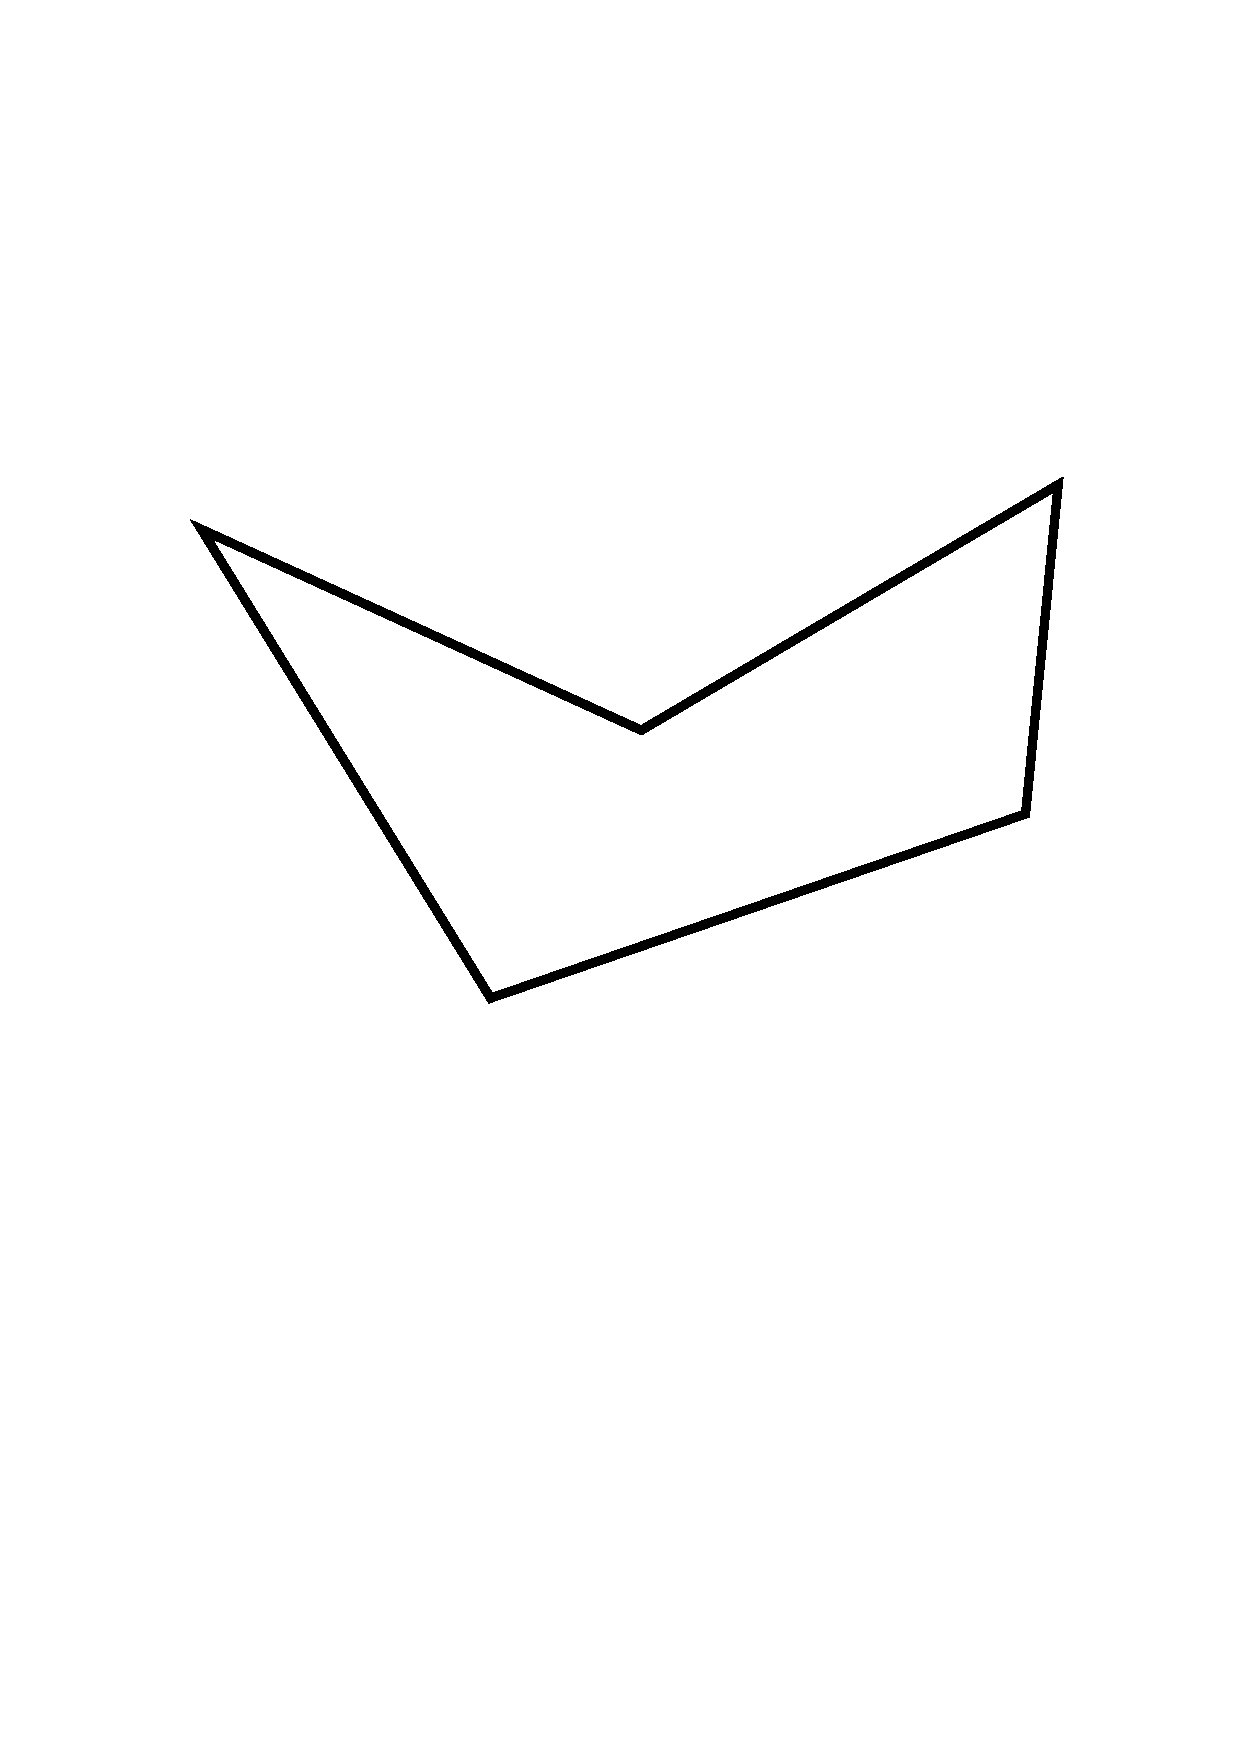
\includegraphics[width=\textwidth]{background/blank-polygon}
    		    \caption{A simple polygon.}
 		 \label{fig:polygon}
	 \end{subfigure}
	 \hspace{.5cm}
	 \begin{subfigure}[b]{0.25\textwidth}
       		  \includegraphics[width=\textwidth]{background/interior-exterior}
     		    \caption{Angles}
 		 \label{fig:interior-exterior}
       \end{subfigure}
        \hspace{.5cm}
     \begin{subfigure}[b]{0.27\textwidth}
       		  \includegraphics[width=\textwidth]{background/exterior-angles-polygon}
       		  \caption{Exterior angles.}
       		   \label{fig:exterior-angles}
         \end{subfigure}
		\caption{(\subref{fig:polygon}) A simple polygon $P.$
		(\subref{fig:interior-exterior}) The interior and exterior angles formed at a vertex.
 		 (\subref{fig:exterior-angles}) The sum of the exterior angles of a simple
		polygon is $2\pi$. Here
		$\beta_1+\beta_2+\beta_3+\beta_4+\beta_5=2\pi$ note that $\beta_4$ is negative.
 		\label{fig:simple-polygon}}
 \end{figure}

If we extend one of the sides of $P$ two complementary angles appear.
The angle inside $P$ is the \EMPH{interior} angle and the complement 
is the  \EMPH{exterior angle}. An example is shown in \figref{interior-exterior}.
We differentiate between turning left and right.
Vertices with interior angles  greater than $\pi$ are called \EMPH{reflex}, see \figref{exterior-angles}. 
At reflex vertices exterior angle is negative.



We now state a simple version of the Gauss-Bonnet theorem \cite{gottlieb_all_1996,polya_elementary_1954},

\begin{theorem}[Gauss-Bonnet for Polygons in the Plane]\label{thm:simple-bonnet}
Let $P$ be a simple polygon in the plane with $n$  vertices,
interior angles $\{\alpha_1,\alpha_2,\ldots,\alpha_n\}$
and exterior angles $\{\beta_1,\beta_2,\ldots,\beta_n\}$ then
$$\sum_{i=1}^n\beta_i=2\pi$$
and 
$$\sum_{i=1}^n\alpha_i=\pi(n-2).$$
\end{theorem}


\begin{proof}

	We traverse a polygon and rotate $\beta_i$ at each vertex
	when we get back to where we started we will have preformed 
	one complete revolution so $\sum_{i=1}^n\beta_i=2\pi.$
	The exterior angles are complementary to the interior angles
	so for each $i$ we have $\beta_i=\pi-\alpha_i$  and using the first
	part of the theorem,  we have
	$\sum_{i=1}^n(\pi-\alpha_i)=n\pi -\sum_{i=1}^n\alpha_i=2\pi$. 
	Solving for $\sum_{i=1}^n\alpha_i$ gives the second part of the theorem.

\end{proof}
No matter how we position the vertices of our polygon,
if the boundary of the polygon stays closed and simple,
the sum the exterior angles will be $2\pi$.
Even this simple version of the Gauss-Bonnet theorem has powerful
consequences, as we now see in our first application, a proof of Pick's Theorem.





\subsection{Pick's Theorem}
\label{sec:pick}

Pick's Theorem gives a formula for the area of a polygon
in the plane with vertices on the lattice $\ZZ^2$ \cite{og-pick}.
We give a proof originally due to Blatter \cite{blatter_another_1997}
and restated by Tabachnikov  \cite{tabachnikov_proofs_2014}.

\begin{theorem}[Pick's Theorem]\label{thm:pick}
Let $P$ be a simple polygon in the plane with vertices on the lattice $\ZZ^2$,
let $I$ be the number of lattice points inside of $P$, let $B$ be the number
of lattice points on the boundary of $P$ and let $A$ denote the area of $P$.
Then, 
$$A=I+\frac{B}{2}-1.$$
\end{theorem}
See \figref{picks} for an example.

 \begin{figure}[htb]
         \centering
         \includegraphics[width=5cm]{pick}
	\caption{A polygon with vertices on the lattice. 
	There are 10 interior vertices and 12 vertices on the boundary.
	By Pick's theorem the area of the polygon is $10+\frac{12}{2}-1=15.$
	\label{fig:picks}}
 \end{figure}
 
\begin{proof}
	Put a unit volume ice cube at each lattice point in the plane and let the ice melt.
	The water will evenly cover the plane with the amount of water inside the polygon 
	equal to its area.
	
	Consider a edge on the the polygon. The amount of water that flows
	into to polygon across this edge equals that amount of water that flows out of the polygon
	across this edge by symmetry. This is because the edge connects two lattice points,
	for each point the contributes flow across the edge in one direction there is a symmetric
	point that contributes and equal amount of flow in the opposite direction.
	So, the total flow across each edge is zero and
	the  amount of water inside the polygon comes from interior cubes and the lattice vertices
	of the polygon.
	
	Each interior lattice point contributes one unit of water. 
	Each lattice point on an edge, half of the water flows into the polygon and
	half flows outside of the polygon.
	Let $\alpha_i$ denote the interior angles at each vertex.
	Each vertex contributes $\frac{\alpha_i}{2\pi}$ units of water to the area.
	By the Gauss-Bonnet theorem, \thmref{simple-bonnet}, the sum of the interior
	angles is $\pi(n-2)$. Thus, the vertex points contribute a total of 
	$$\frac{\pi(n-2)}{2\pi}=\frac{n}{2}-1.$$
	The theorem follows.

\end{proof}






\section{Polygonal Meshes}
\label{sec:polygonal}

In this section, we introduce polygonal meshes, describe a data structure to efficiently
work with them, and define the Euler characteristic.

\subsection{What is a surface?}

 Many surfaces are made up of many vertices, edges, and
triangles (or other polygons). We denote the set of vertices, edges and faces in a triangulated surface as 
$V, E$ and $F$ respectively. We call such a surface a \emph{mesh}
or triangulated mesh, if all faces are triangles.
An example of a triangular mesh is shown in \figref{cat},
notice that this mesh has a boundary on the collar, eyes, and mouth.
Let $\partial(V)$ denote vertices on the boundary of a surface and let $V_{int}$ 
denote vertices that are not on the boundary.



 \begin{figure}[htb]
         \centering
        \begin{subfigure}[b]{0.3\textwidth}
         \includegraphics[width=\textwidth]{polygonal-mesh/profile}
         \caption{}
 	 \label{fig:profile}
       \end{subfigure}
         \hspace{.6cm}
         \begin{subfigure}[b]{0.19\textwidth}
         \includegraphics[width=\textwidth]{polygonal-mesh/head-on}
         \caption{}
          \label{fig:head-on}
         \end{subfigure}
             \hspace{.6cm}
         \begin{subfigure}[b]{0.24\textwidth}
         \includegraphics[width=\textwidth]{polygonal-mesh/back}
         \caption{}
          \label{fig:back}
         \end{subfigure}
		\caption{(\subref{fig:profile}) A profile view of a mesh.
 		(\subref{fig:head-on})  A head on view of the same mesh and the view from the back (\subref{fig:back}).
 		\label{fig:cat}}
 \end{figure}

One way to store a mesh in a computer is as a OFF file.
The first optional line of an OFF file identifies the file as an OFF file.
The second line lists the number of vertices, faces, and edges.
A list of vertices in $(x,y,z)$ coordinates is then given followed
by a list of faces indicated by the index of the vertices contained in the face.
For the mesh in \figref{cat}, the OFF file looks is shown in 
\tabref{off}.

\begin{table}[h!]
\caption{The OFF data for the mesh in \figref{cat}.}
\centering
\begin{tabular}{|p{2cm} p{2cm} p{2cm} p{2cm}|} 
 \hline
\texttt{OFF} &  & &  \\ 
\texttt{7529} & \texttt{14859} & \texttt{0} &  \\ 
\texttt{-0.29196} & \texttt{-0.0867173} & \texttt{-0.355149}  &  \\
 \texttt{-0.123586}   & \texttt{-0.0127199} & \texttt{-0.385597} &  \\
\texttt{-0.138255}   & \texttt{-0.0985078} & \texttt{-0.384018} &  \\
  & &\vdots &  \\  
 \texttt{3}&  \texttt{97} &\texttt{1893}& \texttt{1895}\\
 \texttt{3}& \texttt{71} & \texttt{1894} & \texttt{1893} \\
 \texttt{3} & \texttt{16} & \texttt{1895} & \texttt{1894}\\
   & &\vdots &  \\  
 \hline
\end{tabular}

\label{tab:off}
\end{table}

Suppose we work in a machine shop and a customer has an metal object that they would like
to duplicate.
One way to do this, is by 3D scanning the object to capture the coordinates on the 
surface and represent the object as a triangulated mesh, then use a machine to carve the object
from a block of metal. 
While scanning, errors might occur. As a result of these errors
we might obtain a triangulation that intersects itself. If we try to reconstruct the object
from our mesh our machines will have ambiguous information of what the surface of the object
should be.
This motivates developing an algorithm to determine if a mesh has self-intersections.
Determining if two faces intersect using the OFF representation of a surface is combersome.
To simplify algorithms on meshes we load the OFF file into a more convenient data-structure,
the doubly-connected edge list.

The doubly-connected edge list (DCEL) consists of three separate and related structures, one each
for the vertices, edges, and faces \cite{dutchbook3}.
For each edge, we store two directed half-edges $(\overrightarrow{e})$, with pointers to: its origin, the twin half-edge, the incident face that it bounds, the next half-edge bounding the same face, and the previous half-edge bounding the same face.



\subsection{The Euler Characteristic}

The \EMPH{Euler Characteristic} of a surface $\chi$ is the 
the number of vertices minus the number of edges plus  the number of faces, $\chi=|V|-|E|+|F|.$
In higher dimensions, for a triangulated space $X$ the Euler characteristic is 
$\chi(X)=k_0-k_1+k_2-k_3+\ldots$ where $k_n$ is the number of `triangles' of dimension $n.$
The Euler characteristic is a topological invariant of a space
and does not depend on the choice of triangulation.

A  graph  is \EMPH{planar} if it can be drawn in the plane with intersections only occurring
at vertices.
Two dimensional spheres $\Sp^2$ and two dimensional disk $D^2$ 
will be used in our applications.
For the sphere, we have $\chi(\Sp^2)=2$ 
several proofs of this can be found on David Eppstein's website \cite{eppstein-proofs}.




We include the following proof Thurston \cite{thurston}. 
For any planar graph we can map the graph on to the two sphere using stereographic projection.
 

\begin{theorem}[Euler Characteristic for Planar Graphs]\label{thm:euler}
For any planar graph on the 2-sphere we have $V-E+F=2.$
\end{theorem}

\begin{proof}
If needed, perturb the triangulation so that the north and south poles are 
inside of a two faces and there are no vertical edges. At each vertex place a unit positive
charge, at the center of each edge place a unit negative charge and put a unit positive
charge in the middle of each face. Slam the sphere on the ground so that all charges
on the edges and vertices are moved into the face below them. For faces that do not contain a pole
the net charge will be zero, the northern boundary consists of an alternating sequence
of edges and vertices  beginning  and ending with an edge.
The face containing the north pole has a unit positive charge, and the face containing the south
pole contains positive four units of charge and negative three units of charge.
Thus, the total charge is two.

\end{proof}

Triangulations of the sphere are a special case of \thmref{euler}.
The sphere will be one of two common surfaces we see in applications
of the Gauss-Bonnet theorem. The other being the disk.
For the disk, $\chi(D^2)=1$. This can be seen by considering
the removal of a single face from a triangulation of the sphere.
Once a face is removed, we can project the remaining faces of the sphere
onto the plane to obtain a triangulation of a disk. Moreover, this projection
is invertible and given a triangulation of a disk we can obtain a triangulation
of the sphere with a single face omitted.

The Euler characteristic of a connected, orientable surface surface is often 
stated in terms of the genus of the surface which is defined as follows.
\begin{definition}[Genus of a Surface]\label{def:genus}
	The genus of a connected, orientable surface is the maximum number of
	cuttings along non-intersecting simple closed curves without disconnecting
	the surface \cite{munkres}.
\end{definition}


For an orientable surface, the genus and the Euler characteristic are related by
the formula $\chi=2-2g$. To see this, we can transform a triangulation of a surface of
genus $g$ into a surface of genus $g+1$ by removing two faces and an equal number
of vertices and edges. \figref{genus} provides an example.
Thus, the sphere has genus zero and the torus has genus one.


\begin{figure}[htb]
        \centering
        \begin{subfigure}[b]{0.2\textwidth}
        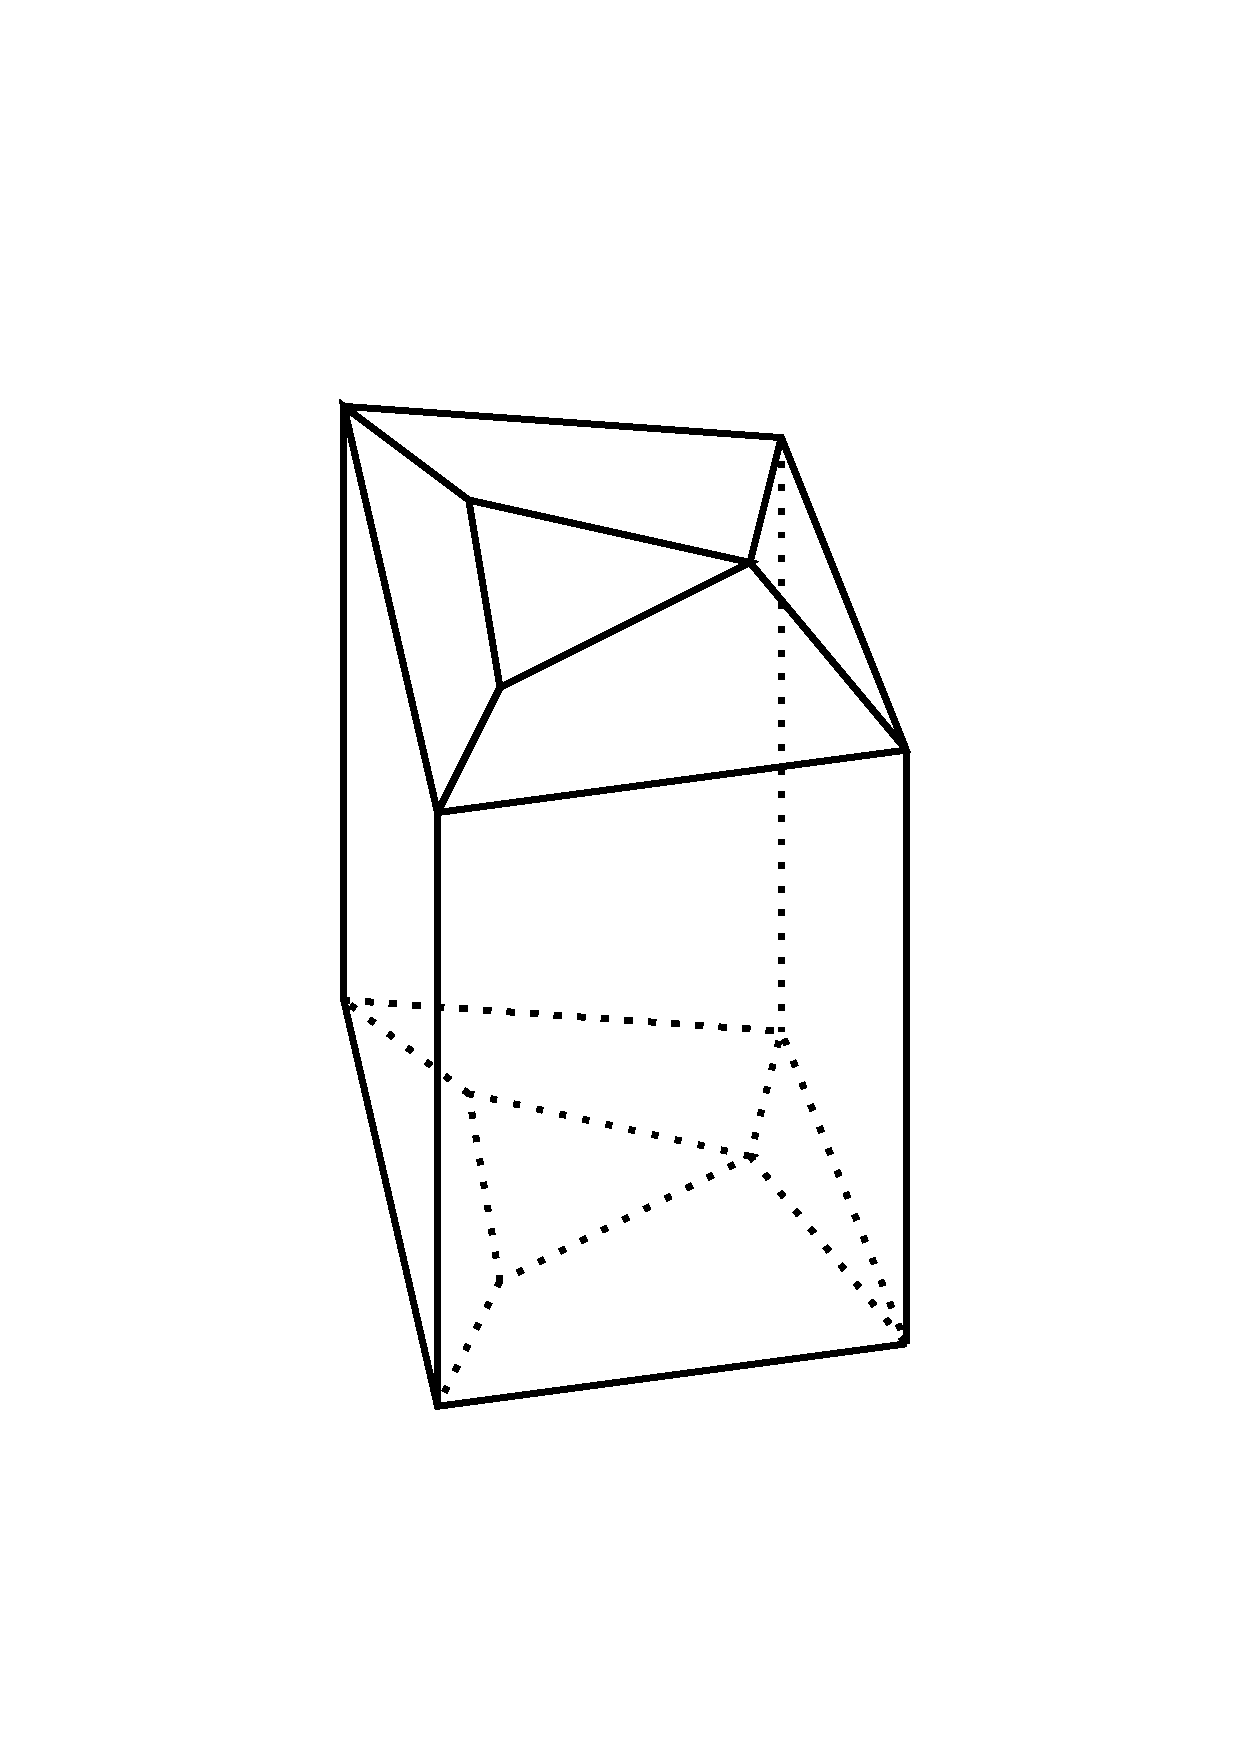
\includegraphics[width=\textwidth]{genus/genus-1}
        \caption{Genus zero.}
          \label{fig:initial-sphere}
        \end{subfigure}
          \hspace{.5cm}
         \begin{subfigure}[b]{0.2\textwidth}
        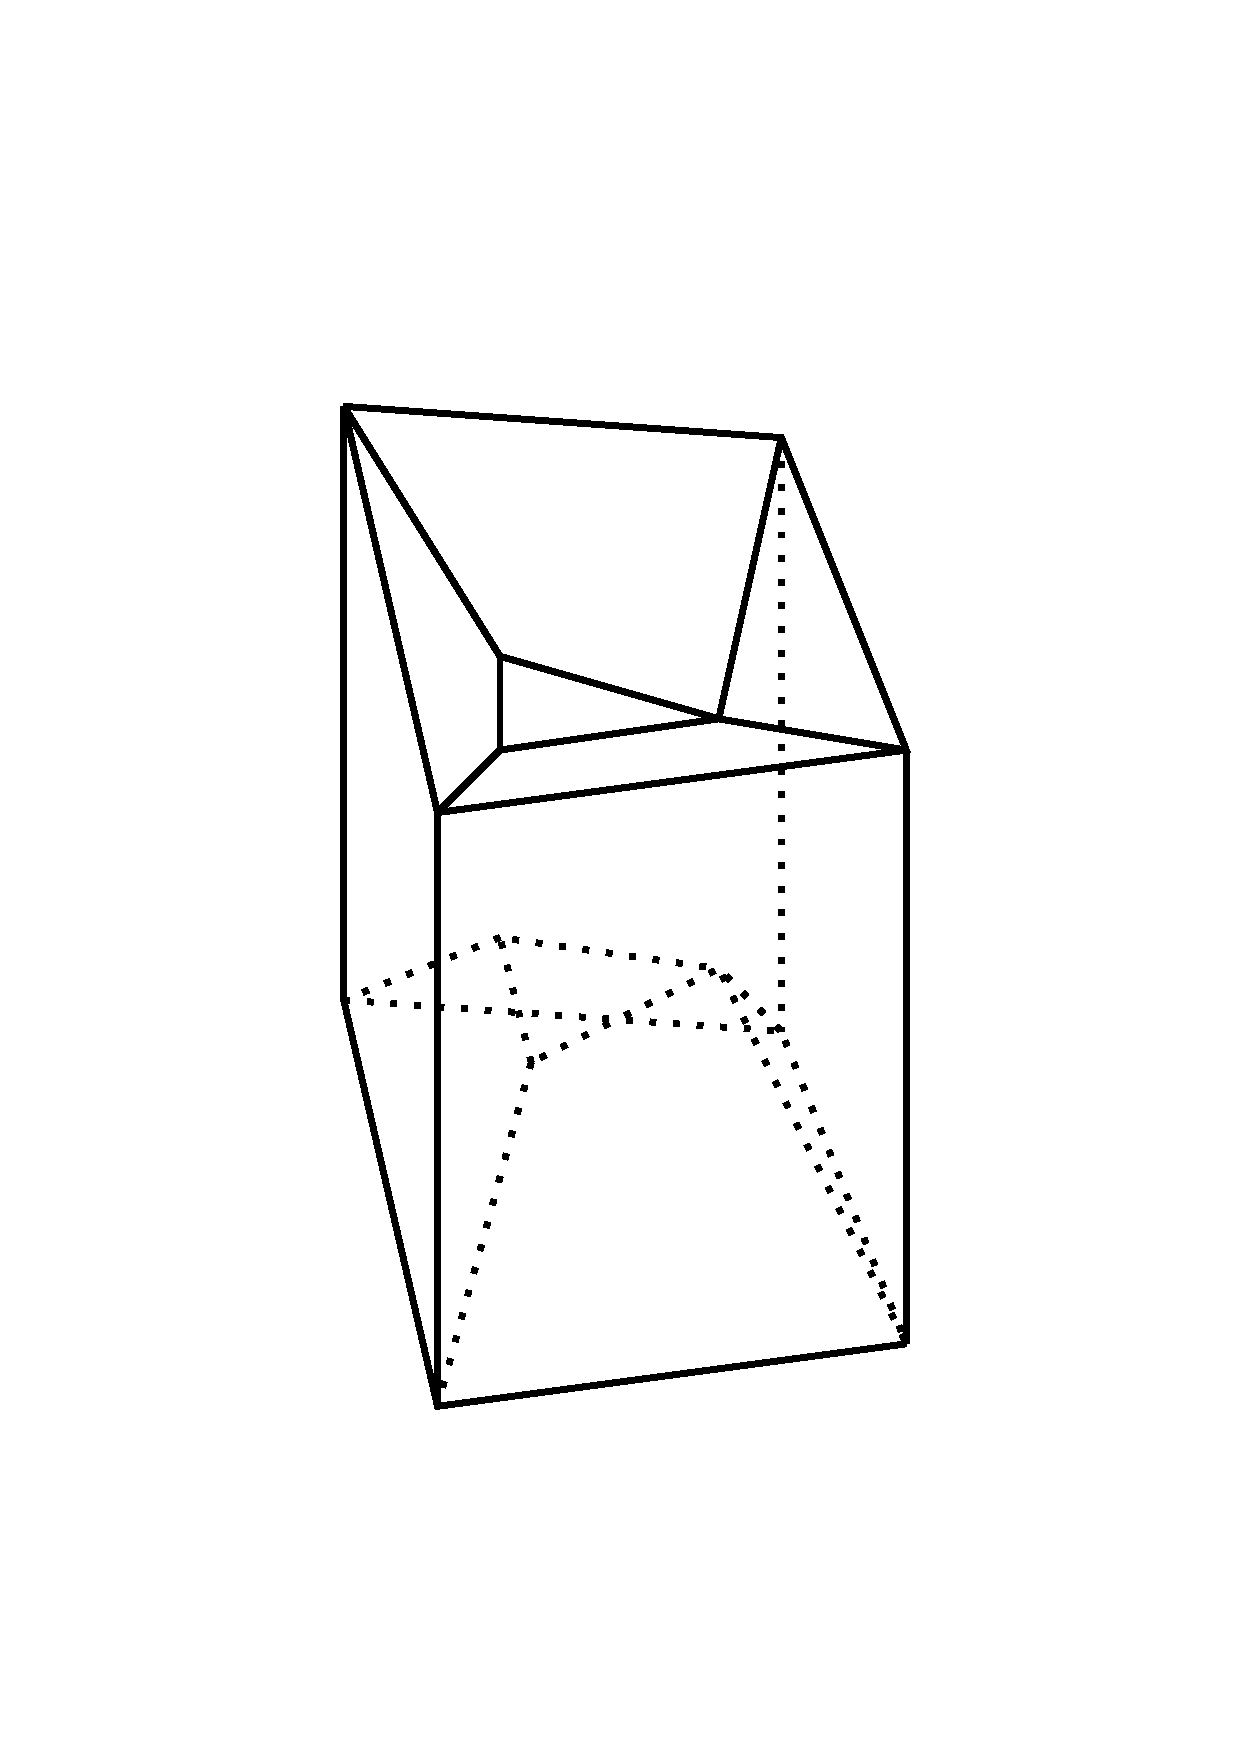
\includegraphics[width=\textwidth]{genus/genus-2}
        \caption{Deform.}
        \label{fig:decending-faces}
        \end{subfigure}
          \hspace{.5cm}
         \begin{subfigure}[b]{0.2\textwidth}
        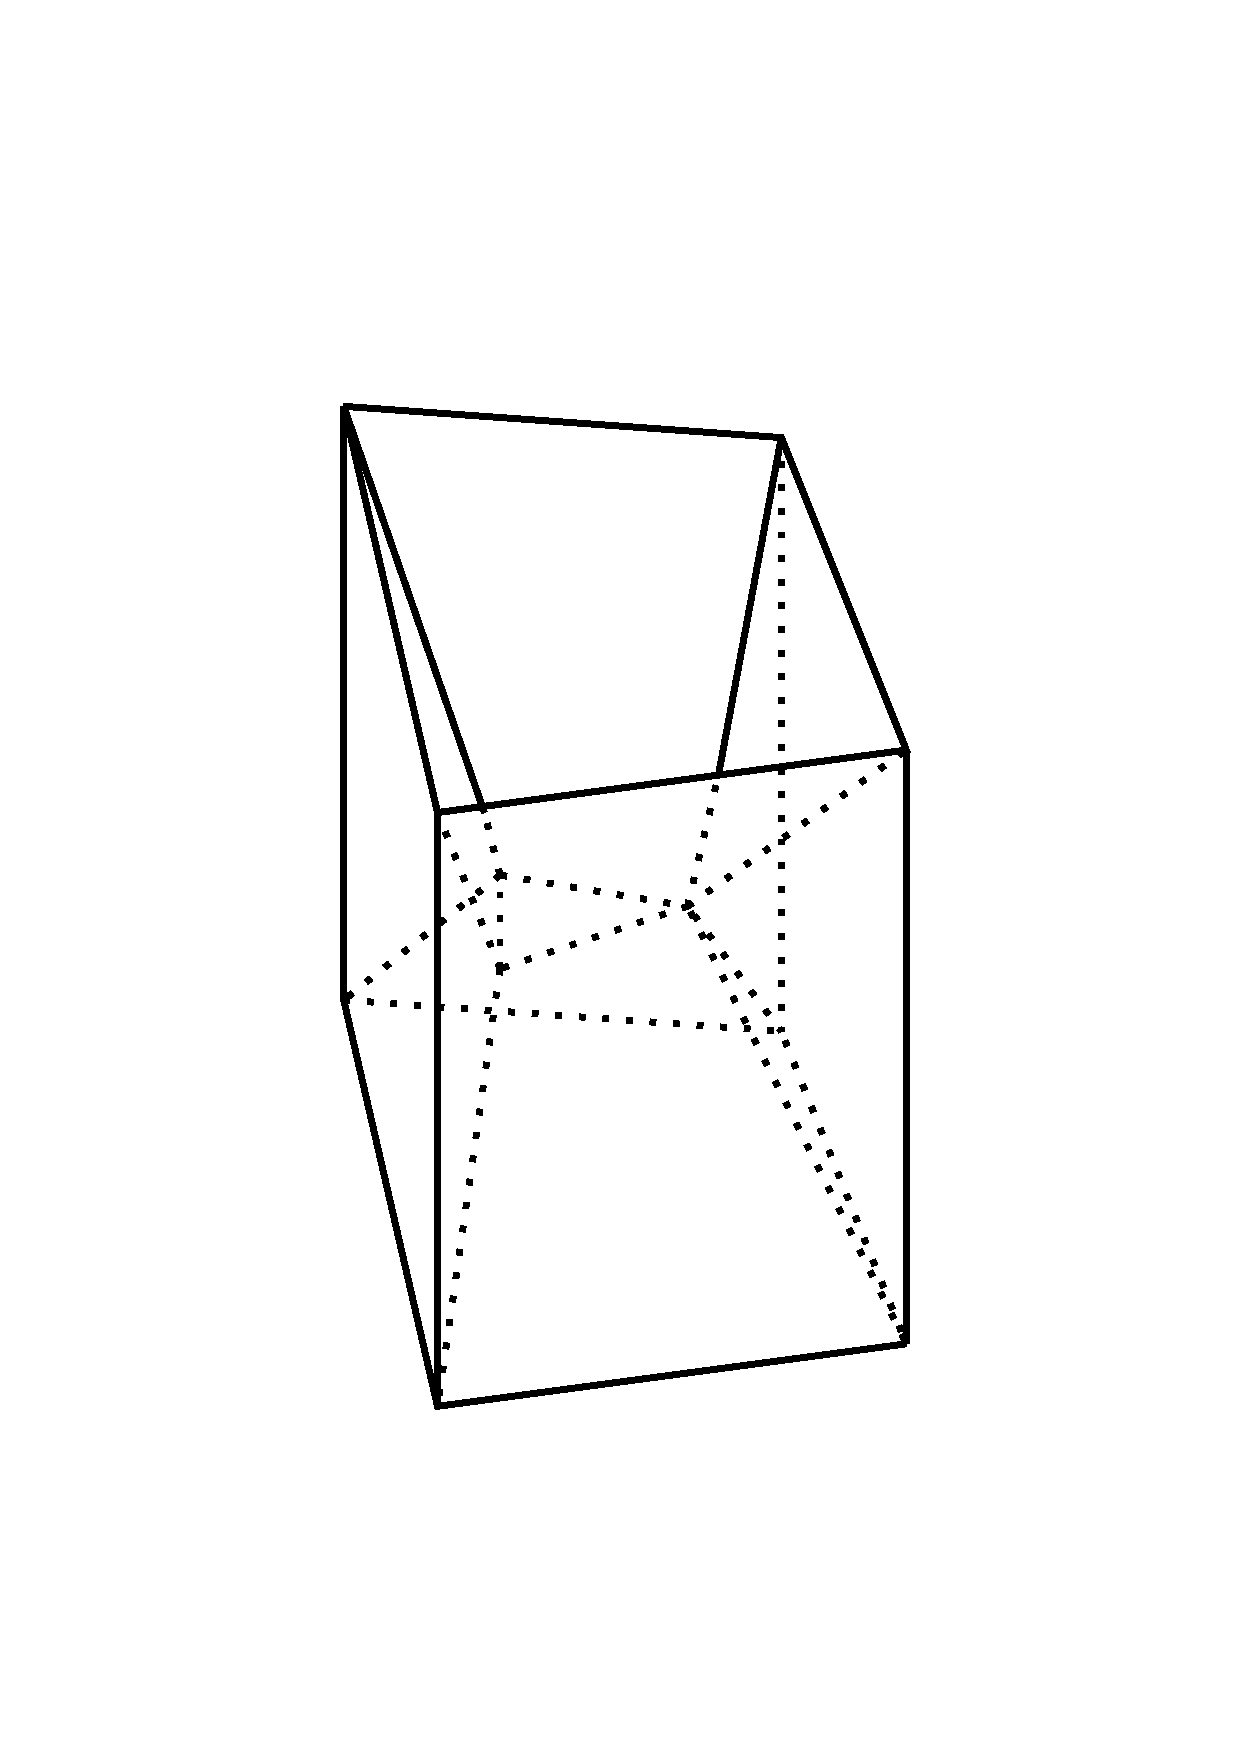
\includegraphics[width=\textwidth]{genus/genus-3}
        \caption{Triangles join.}
        \label{fig:faces-join}
        \end{subfigure}
		\caption{(\subref{fig:initial-sphere}) A surface homeomorphic to the sphere with genus zero.
		(\subref{fig:decending-faces}) The triangle on the top and the triangle on the bottom are getting
		closer. (\subref{fig:faces-join})  A surface homeomorphic to the torus. The triangle on the top
		and the triangle on the bottom have been removed. Three vertices and three edges are				removed. The Euler characteristic decreased by two.
		\label{fig:genus}}
\end{figure}

\noindent \textbf{Exercises}


\begin{enumerate}
	\item 
	
\end{enumerate}

\pagebreak
%\section{Introduction}
\label{sec:intro}

\subsection{A Great Theorem}
The Gauss-Bonnet theorem relates the curvature, a local property, of a surface to the 
to the Euler characteristic, a global property. In symbols 

\begin{equation}\label{eqn:g-b-noboundary}
		\int_MK dA =2\pi \chi(M)
\end{equation}
where $M$ is a smooth surface in $\RR^3$ without bounary, $K$ is Gaussian curvature
and $\chi(M)$ is the Euler characteristic of $M$.
The theorem is a bridge between many ideas that may
seem separate at first, see \figref{bridge}. 




\begin{figure}[htb]
\centering
\includegraphics[width=.3\textwidth]{curvature/bridge}
\caption{The Gauss-Bonnet theorem is a star.}
\label{fig:bridge}
\end{figure}

In the book \emph{Using the Borsuk-Ulam Theorem}
\cite{jm08},
Matou\v{s}ek states that a theorem is a great theorem if there are
\begin{enumerate}[(1)]
\item several different equivalent versions,
\item many different proofs,
\item a host of extensions and generalizations, and
\item numerous interesting applications.
\end{enumerate}

By this criteria, the Gauss-Bonnet theorem is a great theorem.
For (1), six\todo{verify} different versions of the theorem are discussed
in \cite{wu_historical_2008}. 
In addition to the version for smooth surfaces given in \eqnref{g-b-noboundary},
we highlight
 several discrete versions for triangulated surfaces. 
  




 
 
As for (2), several fundamentally different proofs exist.  
One common approach is to first prove the theorem for simply connected domains
with boundary, then triangulate a surface and add up the contribution from each triangle.
However, this proof seems to lack a geometric intuition that other proofs provide. \cite{wu_historical_2008},
A second commonly seen proof is to use Stokes theorem  \cite{doc76,pressley_elementary_2010}.
Many other proofs exist \cite{guillemin_differential_2010,levi-bicycle,grinfeld_introduction_2013}.


For (3), the theorem has been generalized in many ways.
The two notable examples are the Chern-Gauss-Bonnet theorem\cite{chern_simple_1944} and
the Atiyah–Singer index theorem is an example  \cite{atiyah_index_1963}.
A generalization to higher dimensions \cite{guillemin_differential_2010}.


As for (4), applications, 
seven are given in \cite{doc76}.
For applications to physics see \cite{tirado-physics-apps,gibbons_applications_2008}.
This work provides many examples related to the algorithms and combinatorics. 
I hope that the number of applications continues to grow,
please share any that you feel
ought to be included\footnote{\text{bradleymccoy@montana.edu}}.


\subsection{Simple Polygons}
\label{sec:warm-up}

To get a sense of the types of problems we will encounter,
we begin by deriving a formula for the area
of a simple polygon on the sphere in terms of the 
interior angles.
\begin{theorem}\label{thm:triangle}
In the plane, the sum of the interior angles of a triangle is $\pi$.
\end{theorem}
\begin{proof}
Draw a line parallel to one edge through the opposite vertex.
By alternating interior angles in the plane, the sum of the angles
in the triangle equal  a straight line.
See \figref{angles} for an illustration. 



\begin{figure}[htb]
\centering
\includegraphics[width=.3\textwidth]{background/interior-angles-triangle}
\caption{A proof that, in the plane, the sum of the angles of a triangle is $\pi$.}
\label{fig:angles}
\end{figure}

\end{proof}



Consider any simple polygon in the plane $P$ with $n$ vertices. 
Then $P$ can be triangulated with $n-2$ triangles \cite{orourke_computational_1994}.
Thus, when we traverse $P$ we go around $n-2$ triangles each contributing
$\pi$.
We have
\begin{corollary}\label{cor:angles}
In the plane, any simple polygon $P$ with $n$ vertices,
the sum of the interior angles of $P$ is $(n-2)\pi$.

\end{corollary}

Now consider a triangle on the two dimensional sphere as in \figref{sphere-triangle}.

\begin{figure}[htb]
\centering
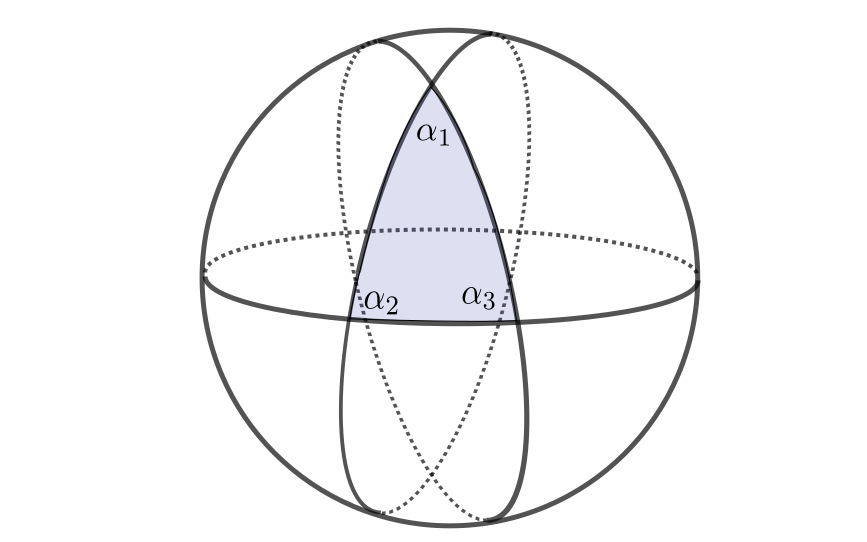
\includegraphics[width=.5\textwidth]{background/sphere-triangle}
\caption{A triangle on the sphere.}
\label{fig:sphere-triangle}
\end{figure}


\begin{figure}[htb]
\centering
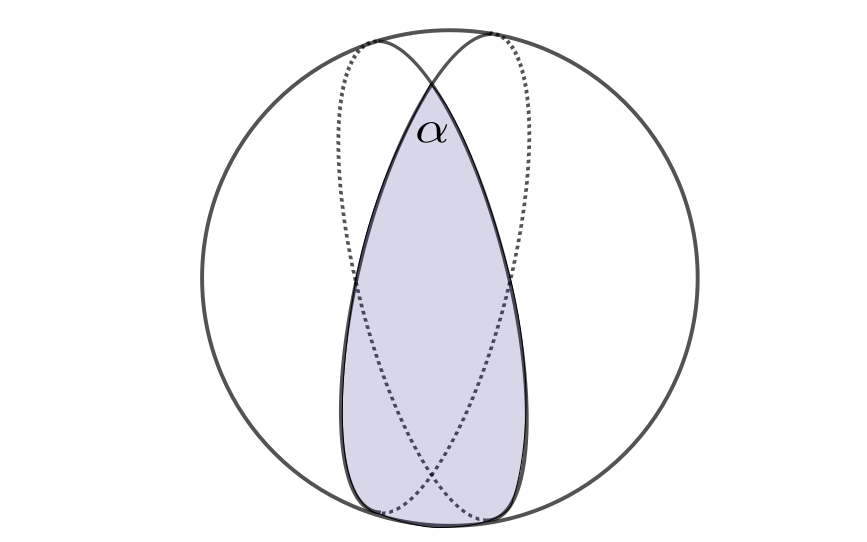
\includegraphics[width=.4\textwidth]{background/lune}
\caption{A lune with angle $\alpha$.}
\label{fig:lune}
\end{figure}

\subsection{Pick's Theorem}
\label{sec:pick}

\cite{og-pick}
\cite{blatter_another_1997}
\cite{tabachnikov_proofs_2014}



\section{The Plane and the Sphere}
\label{sec:plane-sphere}


The sphere and the plane are two surfaces that we will
frequently encounter. 
Stereographic projection, shown in \figref{stereo1}, is a map between almost all of the sphere
and the plane.
In order to gain intuition we first consider the one dimensional version of stereographic
projection between almost all of the circle and the real line.

\begin{example}[Stereographic Projection \cite{christian-notes}]\label{ex:stereo}
Consider the two sphere with the north pole removed $\Sp^2 \setminus (0,0,1)$,
stereographic projection is a bijection between the points on $\Sp^2 \setminus (0,0,1)$ to the $\R^2$.
Consider a line from the north pole $(0,0,1)$ that intersects $(x,y,z)\in \Sp^2$ parametrized by 
$p(t)=(1-t)(0,0,1)+t(x,y,z)$. By considering the $z$ coordinate we determine the $t$ value where this line
intersects $\R^2$, namely $t=\frac{1}{1-z}.$
This gives the desired map shown in  and in equation form
$$p(x,y,z)\to \left(\frac{x}{1-z},\frac{y}{1-z}\right).$$
\end{example}

\begin{figure}[htb]
	\centering
	\includegraphics[width=.3\textwidth]{curvature/stereo}
	\caption{A point on the sphere is mapped to a point on the plane by stereographic projection.}
	\label{fig:stereo1}
\end{figure}
	

\section{Cast of Characters}

In the plane, if one scales a polygon, the area of the polygon changes
but the angles of the polygon do not.
On the unit sphere, we can relate the area of a simple polygon 
to the angles. This is because the sphere is curved.
A triangle on the sphere is shown in \figref{sphere-triangle}.


 \begin{figure}[htb]
         \centering
        \begin{subfigure}[b]{0.35\textwidth}
         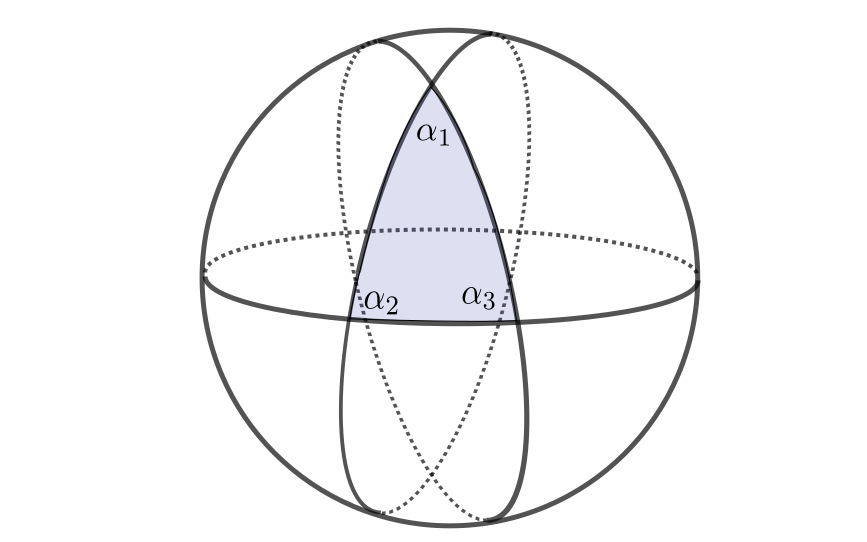
\includegraphics[width=\textwidth]{background/sphere-triangle}
         \caption{Spherical triangle.}
 	 \label{fig:sphere-triangle}
       \end{subfigure}
         \hspace{1cm}
         \begin{subfigure}[b]{0.35\textwidth}
         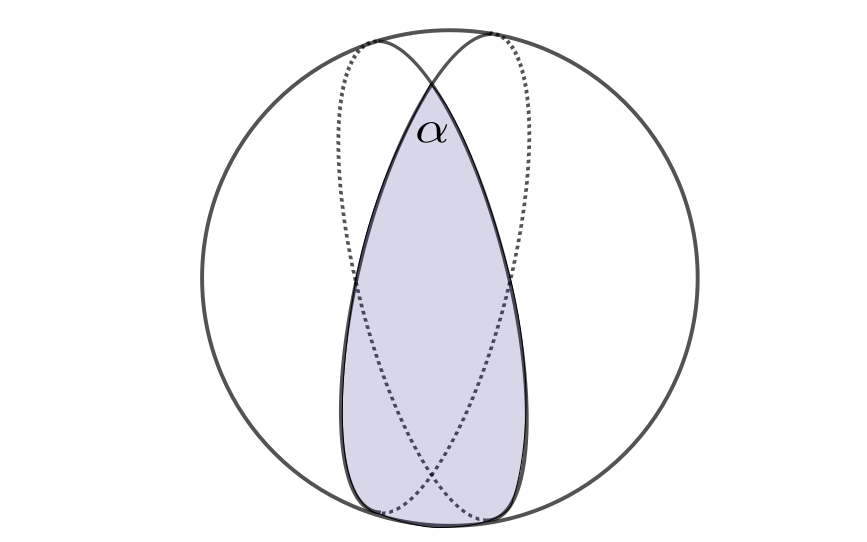
\includegraphics[width=\textwidth]{background/lune}
         \caption{A lune.}
          \label{fig:lune}
         \end{subfigure}
		\caption{(a) A triangle on the sphere.
 		(b) A lune with angle $\alpha$.
 		\label{fig:sphere-lune}}
 \end{figure}
A spherical \EMPH{lune} is the region on a sphere bounded by two half great circles
with angle $\alpha$. The area of a lune is denoted $A(\alpha)$,
 see \figref{lune}.
On the unit sphere, the area of a lune is proportional to $\alpha$. 
If $\alpha=0$ the area is zero and if $\alpha=\pi$ the area is $4\pi$.
We can add the area of two lunes in terms of their angles, 
$A(\alpha_1+\alpha_2)=A(\alpha_1)+A(\alpha_2)$ so $A$ is linear
and  $A(\alpha)=4\alpha.$




The following relates the area of a triangle on the sphere to the angles.

\begin{lemma}[Area of Spherical Triangle]\label{lem:spherical-triangle}
On the unit sphere, the area of a triangle with interior angles $\alpha_1, \alpha_2, \alpha_3$
is $A=\alpha_1+\alpha_2+\alpha_3-\pi$.
\end{lemma}

\begin{proof}
	Any two edges of the the triangle form a lune. The collection of 
	all three lunes covers the entire sphere with triangle and the antipodal triangle covered three times.
 	The surface area of the unit sphere is $4\pi$.
	Thus, $4\pi=4\alpha_1+4\alpha_2+4\alpha_3-4A$
	and $A=\alpha_1+\alpha_2+\alpha_3-\pi$.
\end{proof}

As in the plane, any polygon on the sphere with $n$ vertices can be decomposed
into $n-2$ triangles \cite{orourke_computational_1994}. This gives a formula for the area of a simple polygon
on the sphere with interior angles $\alpha_1,\alpha_2,\ldots, \alpha_n$.

\begin{equation} \label{eqn:sphere-area}
	A=(2-n)\pi +\sum_{i=1}^n \alpha_i.
\end{equation}




This difference between the plane and the sphere illustrates
the need to quantify how much a surface is curving.
What  do we require of a definition of curvature?
A straight line should have zero curvature and
 large circles should have less curvature than smaller circles.
We also need to differentiate between
curving to the left and curving to the right.

For any point on a smooth one dimensional curve in the plane,
we can approximate the curve with a circle.
The best approximating circle is the  \EMPH{osculating circle}.
A natural definition of the \EMPH{curvature} is the inverse of the radius of the osculating
 circle $k=\frac{1}{r}$.
See \figref{osculating-circle} for an example.
The osculating circle meets the requirements for a definition of curvature as long
as we allow the straight line to have an osculating circle with infinite radius.
We determine the sign of the curvature by which side of the curve the osculating circle is on.




The above definition provides great intuition for the curvature of curves
and surfaces.
Computing this value depends on how a curve or surface is represented. 

\begin{figure}[htb]
	\centering
	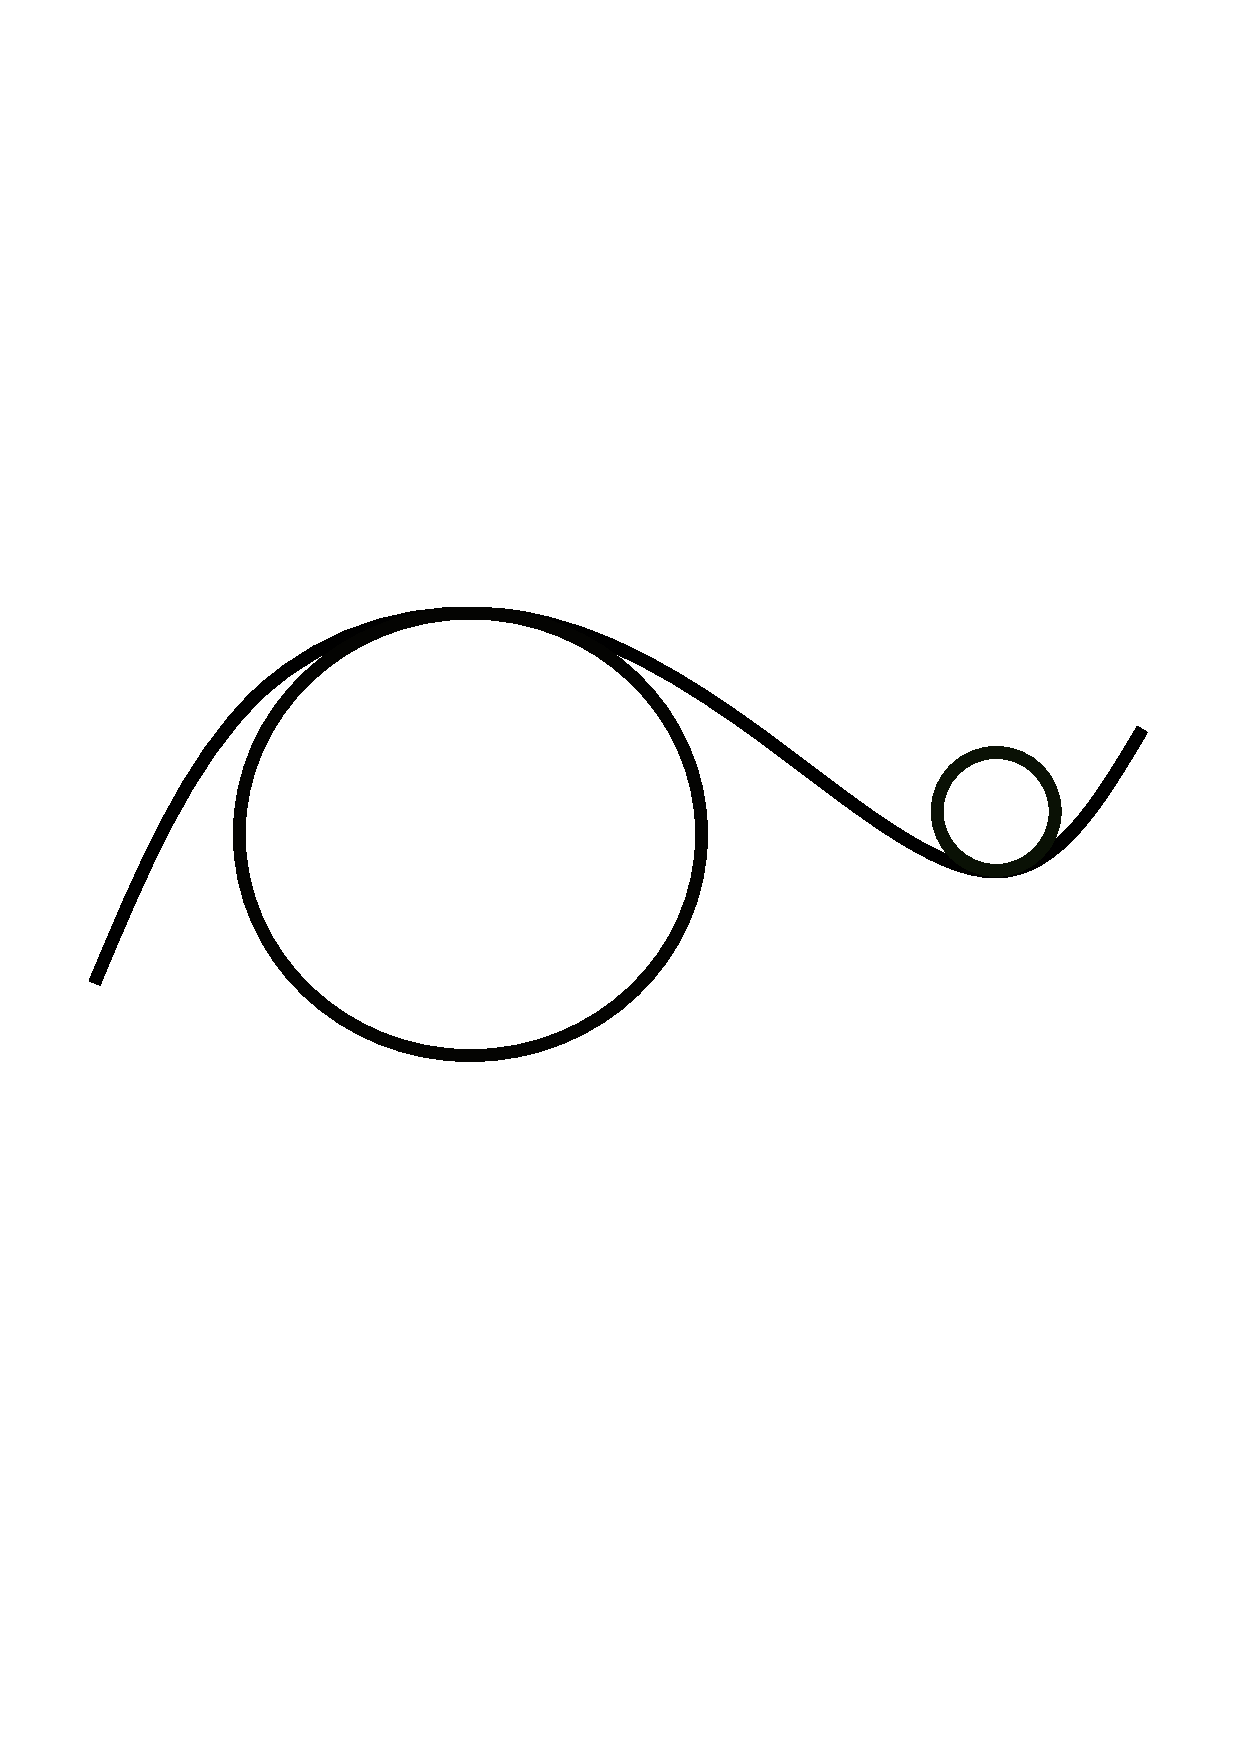
\includegraphics[width=.3\textwidth]{curvature/osculating}
	\caption{A curve with two osculating circles. The curvature at these points
	have opposite sign.}
	\label{fig:osculating-circle}
\end{figure}

A curve in $\RR^3$ is often presented as a function
$\gamma(t)=(x(t),y(t),z(t))$. We say that a curve is \EMPH{smooth} on an open interval $I$
if $\gamma'$ it is continuous and $\gamma'(t)\neq (0,0,0)$ on $I$. 
If $\gamma$ is smooth it has a well-defined unit tangent vector $T(t)=\frac{\gamma'(t)}{|\gamma'(t)|}.$
A second way to define the  \EMPH{curvature} at a point is as the signed magnitude of the rate of change of the 
unit tangent vector

\begin{equation} \label{eqn:kappa}
\kappa= \pm | T'(t)|.
\end{equation}
where $t$ is arc length.

For example, take a circle of radius $r$, parameterized by 
$$C(t)=\left(r\cos(t),r\sin(t),0\right).$$
We have 
$$\frac{dC}{dt}=C'(t)=\left(-r\sin(t),r\cos(t),0\right)$$ and $|C'(t)|=r.$
Then $T(t)=\left(-\sin(t),\cos(t),0\right)$ and
$T'(t)=\left(-\cos(t),-\sin(t),0\right)$.
So, $\kappa(t)=\frac{1}{r}$ and, in this case, our definition of curvature agrees with the
osculating circle intuition given above. 
\eqnref{kappa} can be rewritten in the following more computational friendly form 
\begin{equation} \label{eqn:kappa1}
\kappa(t)=\frac{|\gamma'(t)\times \gamma''(t)|}{|\gamma'(t)|^3}.
\end{equation}

We traverse $\gamma$
at unit speed so that the length of the velocity vector is one, $\gamma'(t)^2=1,$ and by the chain rule, $\gamma'\cdot \gamma''=0$.
This implies $\gamma'$ and $\gamma''$ are orthogonal.
Thus, the
vector $\gamma''=N$ is normal to the $\gamma$. 
By taking the cross product of $N$ and $T$ we obtain a vector $B$ called
the binormal vector.
%The vectors $T,N$ and $B$ form the \EMPH{Fernet frame} of $\gamma$ a $p.$

 This osculating-circle idea can be extend
to  surfaces in $\R^3$, by considering the \EMPH{osculating sphere},
But notice that at saddle points on a surface it is not clear which sphere
best approximates the surface. See \figref{osculating-sphere} for two
equally reasonable ways to approximate a saddle with a sphere.

\begin{figure}[htb]
    \captionsetup[subfigure]{justification=centering}
    \centering
    \begin{subfigure}[b]{0.25\textwidth}
        \includegraphics[width=\textwidth]{curvature/sphere-above-saddle}
       \subcaption{}\label{fig:sphere-above-saddle}
    \end{subfigure}
        \hspace{1cm}
        \begin{subfigure}[b]{0.25\textwidth}
        \includegraphics[width=\textwidth]{curvature/sphere-below-saddle}
        \subcaption{}\label{fig:sphere-below-saddle}
        \end{subfigure}
    \caption{(\subref{fig:sphere-above-saddle}) The osculating sphere above the saddle.
        (\subref{fig:sphere-below-saddle}) The osculating sphere above the saddle.
    }
    \label{fig:osculating-sphere}
\end{figure}



\subsection{Gaussian Curvature}


One dimensional curves are represented by differentiable 
parameterized functions $\gamma:I\subset \RR\to \RR^3$,
we would now like to parameterize a surface.
Similarly, a \EMPH{parameterized surface} $S$ is a collection of maps such that
 for each point $p\in S$ we have a neighborhood $X\subset S$
 and a map $r:U\subset \RR^2 \to X\subset \RR^3$, $r(u,v)=(x(u,v),y(u,v),z(u,v))$
 where
 \begin{itemize}
 \item  $r$ is a homeomorphism
 \item $r$ has derivatives of all orders
 \item every point in $S$ is contained in the domain of at least one map.

\end{itemize}
The maps in the third item are called \EMPH{charts}.
If the differential $dr_q:\RR^2\to \RR^3$ is one-to-one for all $q\in U$ then
we say $r$ is \EMPH{regular}. In other words, let $(u,v)$ be coordinates of $U\subset \RR^2,$
a surface is regular if $\frac{\partial r}{\partial u}$
and $\frac{\partial r}{\partial v}$ are linearly independent for all $p\in U$.
Once we choose a chart we define a clockwise orientation to be positive.
 If the clockwise orientation can be consistently extended to the entire surface, we say
the surface is \EMPH{orientable}.


\begin{example}[The Sphere]\label{ex:sphere-charts}

The unit two sphere $\Sp^2\subset \RR^3$ is the set $\{(x,y,z)\in \RR^3 | x^2+y^2+z^2=1\}.$
We can define six charts to parameterize $\Sp^2$.
For $u,v\in[-1,1]$, we have
$$r_{z}(u,v)=(u,v,\sqrt{1-u^2-v^2}) \hspace{.5cm}  r_{-z}(u,v)=(u,v,-\sqrt{1-u^2-v^2}) \hspace{.5cm}  r_{x}(u,v)=(\sqrt{1-u^2-v^2},u,v) $$
$$r_{-x}(u,v)=(-\sqrt{1-u^2-v^2},u,v) \hspace{.5cm}  r_{y}(u,v)=(u,\sqrt{1-u^2-v^2},v) \hspace{.5cm}   r_{-y}(u,v)=(u,-\sqrt{1-u^2-v^2},v). $$

The chart $r_{z}$ is shown in \figref{sphere-chart}

\begin{figure}[htb]
	\centering
	\includegraphics[width=.4\textwidth]{curvature/sphere-chart}
	\caption{A chart of $\Sp^2$.}
	\label{fig:sphere-chart}
\end{figure}

One can verify that these parameterizations fulfill the requirements
for the sphere to be a regular surface.

\end{example}


A \EMPH{tangent vector} to $S$ at $p$ is a map $\xi:(-\epsilon,\epsilon)\to S$ with $\xi(0)=p$.
The set of all tangent vectors is the \EMPH{tangent plane} and it corresponds to the image
of the differential map $d\phi_q(\RR^2)\subset \RR^3$ (prop. 1 \cite{doc76}).
By choosing two linearly independent paths through $p\in S$ we obtain a basis 
for the tangent
plane and define a normal vector $N$ at $p$.
Every plane containing the normal vector will intersect the surface.
The intersection of the surface and each normal plane is a curve in $\RR^3$
gives a one dimensional curve called the \EMPH{normal section}, see  \figref{normal-sections}
for an example.
Let $\kappa_1$ denote the maximum curvature of all normal sections 
and let $\kappa_2$ denote the minimum. 
The \EMPH{Gaussian curvature} of a point on a surface is
$K=\kappa_1\kappa_2.$
One can check that the Gaussian curvature of the plane is zero and
that larger circles have less curvature than smaller ones.



\begin{figure}[htb]
    \captionsetup[subfigure]{justification=centering}
    \centering
    \begin{subfigure}[b]{0.25\textwidth}
        \includegraphics[width=\textwidth]{curvature/normal-section-max}
       \subcaption{}\label{fig:normal-section-max}
    \end{subfigure}
        \hspace{1cm}
        \begin{subfigure}[b]{0.25\textwidth}
        \includegraphics[width=\textwidth]{curvature/normal-section-min}
        \subcaption{}\label{fig:normal-section-min}
        \end{subfigure}
    \caption{(\subref{fig:normal-section-max}) The osculating sphere above the saddle.
        (\subref{fig:normal-section-min}) The osculating sphere above the saddle.
    }
    \label{fig:normal-sections}
\end{figure}


We now consider computing the Gaussian curvature.
A \EMPH{quadratic form} to be polynomial of degree two, of the form $p(u,v)=c_1u^2+c_2uv+c_3v^2$ 
where $c_i\in R$.
We define a quadratic form, the first fundamental form, using $r(u,v)$.

Let $r(u,v)$ be a parameterized surface.
Let $E=r_u\cdot r_u, F=r_u\cdot r_v$ and  $G=r_v\cdot r_v$.
The \EMPH{first fundamental form}
is the quadratic form $\mathrm{I}=Edu^2+2Fdudv +Gdv^2$.
We summarize the first fundamental form as a matrix $$\mathrm{I}=\begin{bmatrix}
E & F \\
F & G 
\end{bmatrix}.$$
%We get a notion of length in the tangent space, an inner product on $Tp(S)$.
%If $x$ and $y$ are two tangent vectors
%then $$\mathrm{I}(x,y)=x^T\begin{bmatrix}
%E & F \\
%F & G 
%\end{bmatrix}y.$$

The first fundamental form enables us to  compute many interesting
things about our surface including arc length, angles between curves,
and area on a surface.
For example,
given a `small' parallelogram $M$ on $S$ with corners $r(u,v),r(u+\epsilon u, v), r(u,v+\epsilon v)$ 
and $r(u+\epsilon u, v+\epsilon v)$ the rate of change of the area of $M$ is 
$$dA=\sqrt{EG-F^2}dudv.$$
In \exref{stereo}, we will use the first fundamental form to compute the arc length of some curves.


Gauss's Egregious (remarkable) Theorem states that the Gaussian curvature only depends
of the first fundamental form. Thus, curvature can be computed entirely by measuring angles, distance 
and their derivatives without any reference to the way that the surface is embedded in $\R^3.$
Because of this property we say that Gaussian curvature is an \emph{intrinsic} property of a surface.
The Brioschi formula gives the Gaussian curvature using only the first fundamental form
\begin{equation}\label{eq:brioschi}
	K=\frac{\begin{vmatrix}
-\frac{1}{2}E_{vv}+F_{uv}-\frac{1}{2}G_{uu} & \frac{1}{2}E_u & F_u-\frac{1}{2}E_v\\
F_v-\frac{1}{2}G_u & E & F\\
\frac{1}{2}G_v & F & G
\end{vmatrix}-\begin{vmatrix}
0 & \frac{1}{2}E_v & \frac{1}{2}G_u\\
\frac{1}{2}E_v & E & F\\
\frac{1}{2}G_u & F & G
\end{vmatrix}}{(EG-F^2)^2}
\end{equation}



While we can compute Gaussian curvature using only the first fundamental form,
 the second fundamental form is convenient for computations.
To this end, the unit normal vector at $p$ is given by $$n(p)=\frac{r_u\times r_v}{|r_u\times r_v|}.$$
Let $L=r_{uu}\cdot n, M=r_{uv}\cdot n$ and $N=r_{vv}\cdot n$ the
\EMPH{second fundamental form} is $\mathrm{I\!I}=Ldu^2+2Mdudv+Ndv^2$,
in matrix form $$\mathrm{I\!I}=\begin{bmatrix}
L & M \\
M & N 
\end{bmatrix}.$$
%Another inner product is given by $$\mathrm{I\!I}(x,y)=x^T\begin{bmatrix}
%L & M \\
%M & N 
%\end{bmatrix}y.$$
Combining the first and second fundamental forms we have
the \EMPH{Gaussian curvature} of a surface is
\begin{equation}\label{eqn:curve-dets}
 	K=\frac{\det(\mathrm{I\!I})}{\det(\mathrm{I})}.
\end{equation}

\begin{example}[Curvature of the Sphere]\label{ex:compute-surface-curvature}
Consider the northern hemisphere of the unit sphere parameterized
by $$r(u,v)=(u,v,\sqrt{1-u^2-v^2})$$ and we wish to compute the Gaussian curvature at
the north pole $p=(0,0,1)$.
We have $$r_u|_p=(1,0,\frac{-u}{\sqrt{1-u^2-v^2}})|_p=(1,0,0)$$ and
$$r_v|_p=(0,1,\frac{-v}{\sqrt{1-u^2-v^2}})|_p=(0,1,0).$$
We have $E=1, F=0,$ and $G=1$ so our first fundamental form is
$\mathrm{I}=\begin{bmatrix}
1 & 0 \\
0 & 1 
\end{bmatrix}.$
Our normal vector is $n(p)=(0,0,1)$ with 
$$r_{uu}|_p=(0,0,\frac{1-2u^2}{(1-u^2)^{\frac{3}{2}})})|_p=(0,0,1),
r_{uv}|_p=(0,0,0)$$ and 
$$r_{vv}|_p=(0,0,\frac{1-2v^2}{(1-v^2)^{\frac{3}{2}})})|_p=(0,0,1).$$
Thus, $L=1, M=0$ and $N=1$ and our second fundamental form is
$\mathrm{I\!I}=\begin{bmatrix}
1 & 0 \\
0 & 1 
\end{bmatrix}$
and our Gaussian curvature is $K=\frac{\det(\mathrm{I\!I})}{\det(\mathrm{I})}=\frac{1}{1}=1$ as expected.

\end{example}

We will use the first fundamental form to compute
the arc length of circles on the sphere parallel to the $xy$ plane with fixed height $z=c$ for $-1<c<1$.
Stereographic projection, described in \secref{plane-sphere},
allows us map our problem to the plane and perform our computations there.

\begin{example}[Stereographic Projection Revisited\cite{christian-notes}]\label{ex:stereo}
Consider the two sphere with the north pole removed $\Sp^2 \setminus (0,0,1)$,
stereographic projection is a bijection between the points on $\Sp^2 \setminus (0,0,1)$ to the $\R^2$.
Consider a line from the north pole $(0,0,1)$ that intersects $(x,y,z)\in \Sp^2$ parametrized by 
$p(t)=(1-t)(0,0,1)+t(x,y,z)$. By considering the $z$ coordinate we determine the $t$ value where this line
intersects $\R^2$, namely $t=\frac{1}{1-z}.$
This gives the desired map shown in \figref{stereo} and in equation form
$$p(x,y,z)\to \left(\frac{x}{1-z},\frac{y}{1-z}\right).$$

\begin{figure}[htb]
	\centering
	\includegraphics[width=.3\textwidth]{curvature/stereo}
	\caption{A point on the sphere is mapped to a point on the plane by stereographic projection.}
	\label{fig:stereo}
\end{figure}
	
The inverse is given by $p^{-1}:\R^2\to \R^3$

	\begin{equation}\label{eqn:stereo}
		p^{-1}(u,v)=\left(\frac{2u}{u^2+v^2+1},\frac{2v}{u^2+v^2+1},\frac{u^2+v^2-1}{u^2+v^2+1}\right).	
	\end{equation}
To compute the first fundamental form of $p^{-1}(u,v)$ we take the partial derivatives

$$p^{-1}_u=\left(\frac{2v^2-2u^2+2}{(u^2+v^2+1)^2},\frac{-4uv}{(u^2+v^2+1)^2},\frac{4v}{(u^2+v^2+1)^2}\right)$$
and 
$$p^{-1}_v=\left(\frac{-4uv}{(u^2+v^2+1)^2},\frac{2v^2-2u^2+2}{(u^2+v^2+1)^2},\frac{4v}{(u^2+v^2+1)^2}\right).$$
Then, after some algebra,
$$E=p^{-1}_u\cdot p^{-1}_u=\frac{4}{(u^2+v^2+1)^2}$$
$$F=p^{-1}_v\cdot p^{-1}_v=\frac{4}{(u^2+v^2+1)^2}$$
and
$$M=p^{-1}_u\cdot p^{-1}_v=0.$$

We can use the first fundamental form to compute
the arc length of circles on the sphere parallel to the $xy$ plane with fixed height $z=c$ for $-1<c<1$.
This length can be computed using
the pythagorean theorem. We will see that using stereographic projection
and the first fundamental form we get the same answer.


The arc length of a parameterized curve $u=u(t), v=v(t)$ on a regular surface,
can be computed using the first fundamental form.  Let
$s$ denote the arc length, then 
$$ds=\bigg | \frac{dr}{dt}\bigg | dt = \bigg | r_u\frac{du}{dt}+r_v\frac{dv}{dt}\bigg |dt
=\sqrt{(r_u^2 du^2+2r_ur_v du dv + r_v^2dv^2)}.$$
Next, use the map $p$ to map such a circle to the plane.
Using \eqnref{stereo}, our circle on the sphere maps 
to a circle in the plane because
	$$p^{-1}(u,v)=\frac{u^2+v^2-1}{u^2+v^2+1}=c$$
and we can compute the radius in terms of $c$
\begin{equation}\label{eqn:radius}
	u^2+v^2=\frac{1+c}{1-c}=k^2.
\end{equation}
	
In the plane, $u^2+v^2=k^2$ can be parameterized
as $$\gamma(t)=(k\cos(t),k\sin(t))$$ with $0\leq t\leq 2\pi.$
So our curve becomes $p^{-1}\circ \gamma(t)$ on the sphere.
Computing the partial derivatives of $\gamma(t)$ gives
$$\gamma_u'=-k\sin(t)\hspace{1.3cm}  \gamma_v'=k\cos(t).$$
Now we use the first fundamental form

$$\int_{p^{-1}}\gamma ds=\int_{0}^{2\pi} ||(p^{-1}\circ \gamma)'(t)dt=\int_0^{2\pi}\sqrt{E(\gamma_u'(t))^2+2M\gamma_u'\gamma_v'+
F(\gamma_v'(t))^2}dt.$$
Substituting and simplifying using $E=F$ we obtain
$$\int_0^{2\pi}\frac{2k}{k^2+1}dt=\frac{4\pi k}{k^2+1}.$$
Simplifying further using \eqnref{radius}  our arc length is
$$2\pi\sqrt{1-c^2}.$$

\end{example}

Stereographic projection has the property that it preserves the angles.
Maps with this property have a name.
\begin{definition}[Conformal]\label{def:conformal}
	Let $U$ and $V$ be open subsets of $\R^n$, a function $f:U\to V$ is
	\emph{conformal} at a point $u\in U$ if it preserves angles between curves
	through $u$ and preserves orientation.
\end{definition}
Proof that stereographic projection is conformal and circle preserving \cite{hilbert-imagination}.

\begin{theorem}[First Fundamental Form and Conformal Maps]\label{thm:first-conformal}
	Let $S$ be a regular surface and $f:U\subset \R^2 \to V\subset S$ be a chart.
	Let $f$ have first fundamental form $\mathrm{I}=Edu^2+2Fdudv +Gdv^2$.
	Then $f$ is conformal if and only if $E=G$ and $F=0.$
\end{theorem}


\subsection{Geodesics Curvature}

Shortest paths play an important role in many computational problems.
On a surface, a \EMPH{geodesic} is a curve that is a shortest path
between two points in the surface. 
For example, on $\Sp^2$ great circles are geodesic.
Intuitively, the geodesic curvature of a one dimensional curve on a surface
is the curvature as it would be seen from someone living on the surface.


Given a parameterized surface and a point on parameterized curve on the surface,
we can compute the geodesic curvature as follows.
First, find the tangent plane to the surface at the point and the unit normal vector.
Let $U:\mathcal{U}\to \RR^3$ be a parameterized chart on a surface $S$ with vector $n(u,v)$ normal
to the surface
and let $\gamma(\theta)$ be a curve in $U$.
Then $V=n(\gamma(\theta))\times T$ is in the tangent plane of the surface since
it is perpendicular to $n$. Moreover, $V(\theta)$ is normal to $\gamma$ 
from the perspective of someone living on the surface. 
The geodesic curvature tells us the rate of change of $\gamma'$ with respect 
to $V(\theta)$.
The \EMPH{geodesic curvature} is given by 
\begin{equation} \label{eqn:geodesic}
	k_g=\gamma'' \cdot (V\times \gamma').
\end{equation}

\begin{example}[Circles on the Sphere]\label{eqn:circles-on-sphere}
	We can rotate the sphere so that the circle is parallel to the $xy$-plane.
	Then the radius of the circle $r$ is related to the height $h$ of the circle above the $xy$-plane
	by $h^2+r^2=1$. See \figref{geodesic} for an example.
	A parameterization by arc length is given by
	$$\gamma(\theta)=\left(r\cos\left(\frac{\theta}{r}\right),r\sin\left(\frac{\theta}{r}\right),\sqrt{1-r^2}\right),$$
	so
	$$\gamma'(\theta)=\left(-\sin\left(\frac{\theta}{r}\right),\cos\left(\frac{\theta}{r}\right),0\right)$$
	and
	$$\gamma''(\theta)=\left(-\frac{1}{r}\cos\left(\frac{\theta}{r}\right),-\frac{1}{r}\sin\left(\frac{\theta}{r}\right),0\right).$$
	Since we are on the sphere, the normal vector is equal to the point on the sphere
	so $$n(\theta)=\left(r\cos\left(\frac{\theta}{r}\right),r\sin\left(\frac{\theta}{r}\right),\sqrt{1-r^2}\right).$$
	Then 
	$$k_g=\gamma''\cdot V(\theta)=\frac{\sqrt{1-r^2}}{r}.$$
	Notice that if $h=0$ then $r=1$ and the geodesic curvature is zero on the equator.
\end{example}

\begin{figure}[htb]
	\centering
	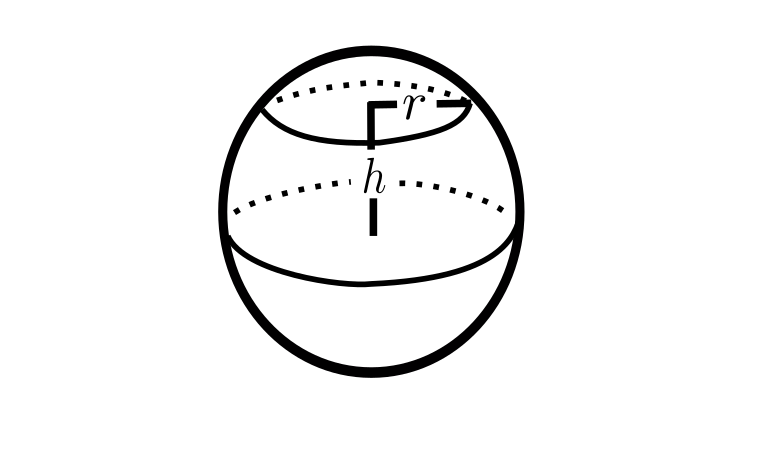
\includegraphics[width=.25\textwidth]{curvature/geodesic}
	\caption{Computing the geodesic curvature.}
	\label{fig:geodesic}
\end{figure}


\subsection{Triangulations and The Euler Characteristic}

We assume the reader is familiar with the notions
of topological spaces and simplicial complexes.
Most introductory topology texts describe these objects \cite{jm08,munkres}.
The applications we will encounter will refer to triangulated surfaces in $\R^3$
called a \EMPH{mesh}, in one application the surface will contain its interior.
Each triangle in a mesh is isomorphic to a triangle in the plane and the sum
of the interior angles is $\pi$.


We denote the set of vertices, edges and faces in a triangulated surface as 
$V, E$ and $F$ respectively.
Let $\partial(V)$ denote vertices on the boundary of a surface and let $V_{int}$ 
denote vertices that are not on the boundary.
See \figref{triangulated-torus} for an example of a triangulated surface.



The \EMPH{Euler Characteristic} of a surface $\chi$ is the 
the number of vertices minus the number of edges plus  the number of faces, $\chi=|V|-|E|+|F|.$
In higher dimensions, for a triangulated space $X$ the Euler characteristic is 
$\chi(X)=k_0-k_1+k_2-k_3+\ldots$ where $k_n$ is the number of simplices of dimension $n.$
The Euler characteristic is a topological invariant of a space
and does not depend on the choice of triangulation.

A  graph  is \EMPH{planar} if it can be drawn in the plane with intersections only occurring
at vertices.
Two dimensional spheres $\Sp^2$ and two dimensional disk $D^2$ 
will be used in our applications.
For the sphere, we have $\chi(\Sp^2)=2$ 
several proofs of this can be found on David Eppstein's website \cite{eppstein-proofs}.




We include the following proof Thurston \cite{thurston}. 
For any planar graph we can map the graph on to the two sphere using stereographic projection.
 

\begin{theorem}[Euler Characteristic for Planar Graphs]\label{thm:euler}
For any planar graph on the 2-sphere we have $V-E+F=2.$
\end{theorem}

\begin{proof}
If needed, perturb the triangulation so that the north and south poles are 
inside of a two faces and there are no vertical edges. At each vertex place a unit positive
charge, at the center of each edge place a unit negative charge and put a unit positive
charge in the middle of each face. Slam the sphere on the ground so that all charges
on the edges and vertices are moved into the face below them. For faces that do not contain a pole
the net charge will be zero, the northern boundary consists of an alternating sequence
of edges and vertices  beginning  and ending with an edge.
The face containing the north pole has a unit positive charge, and the face containing the south
pole contains positive four units of charge and negative three units of charge.
Thus, the total charge is two.

\end{proof}

Triangulations of the sphere are a special case of \thmref{euler}.
The sphere will be one of two common surfaces we see in applications
of the Gauss-Bonnet theorem. The other being the disk.
For the disk, $\chi(D^2)=1$. This can be seen by considering
the removal of a single face from a triangulation of the sphere.
Once a face is removed, we can project the remaining faces of the sphere
onto the plane to obtain a triangulation of a disk. Moreover, this projection
is invertible and given a triangulation of a disk we can obtain a triangulation
of the sphere with a single face omitted.

The Euler characteristic of a connected, orientable surface surface is often 
stated in terms of the genus of the surface which is defined as follows.
\begin{definition}[Genus of a Surface]\label{def:genus}
	The genus of a connected, orientable surface is the maximum number of
	cuttings along non-intersecting simple closed curves without disconnecting
	the surface \cite{munkres}.
\end{definition}

The sphere has genus zero and the torus, shown in \figref{triangulated-torus}, has genus one.
For an orientable surface, the genus and the Euler characteristic are related by
the formula $\chi=2-2g$. To see this, we can transform a triangulation of a surface of
genus $g$ into a surface of genus $g+1$ by removing two faces and an equal number
of vertices and edges. \figref{genus} provides an example.



\begin{figure}[htb]
\centering
\includegraphics[width=.3\textwidth]{background/Torus-triang}
\caption{A triangulation of the torus. Image from wikipedia.}
\label{fig:triangulated-torus}
\end{figure}

\begin{figure}[htb]
        \centering
        \begin{subfigure}[b]{0.2\textwidth}
        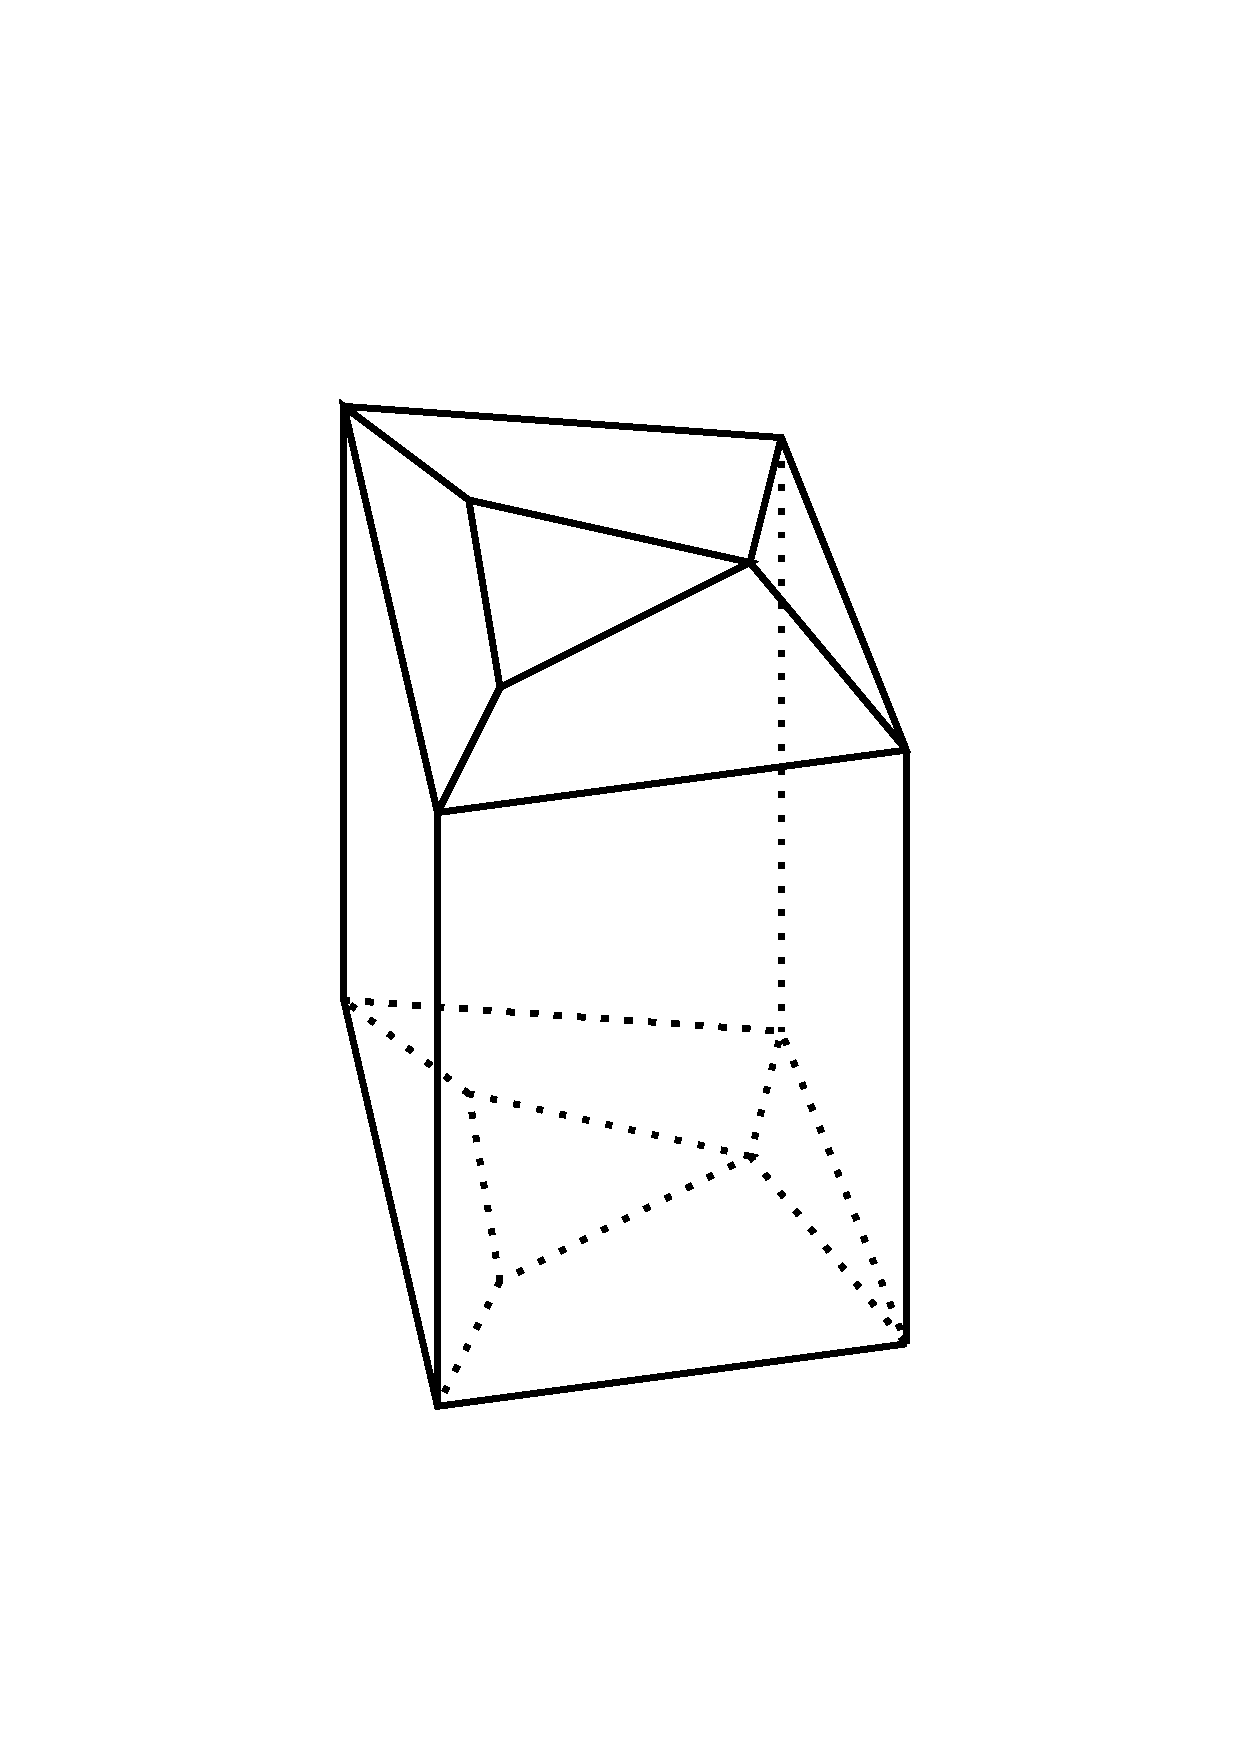
\includegraphics[width=\textwidth]{genus/genus-1}
        \caption{Genus zero.}
          \label{fig:initial-sphere}
        \end{subfigure}
          \hspace{.5cm}
         \begin{subfigure}[b]{0.2\textwidth}
        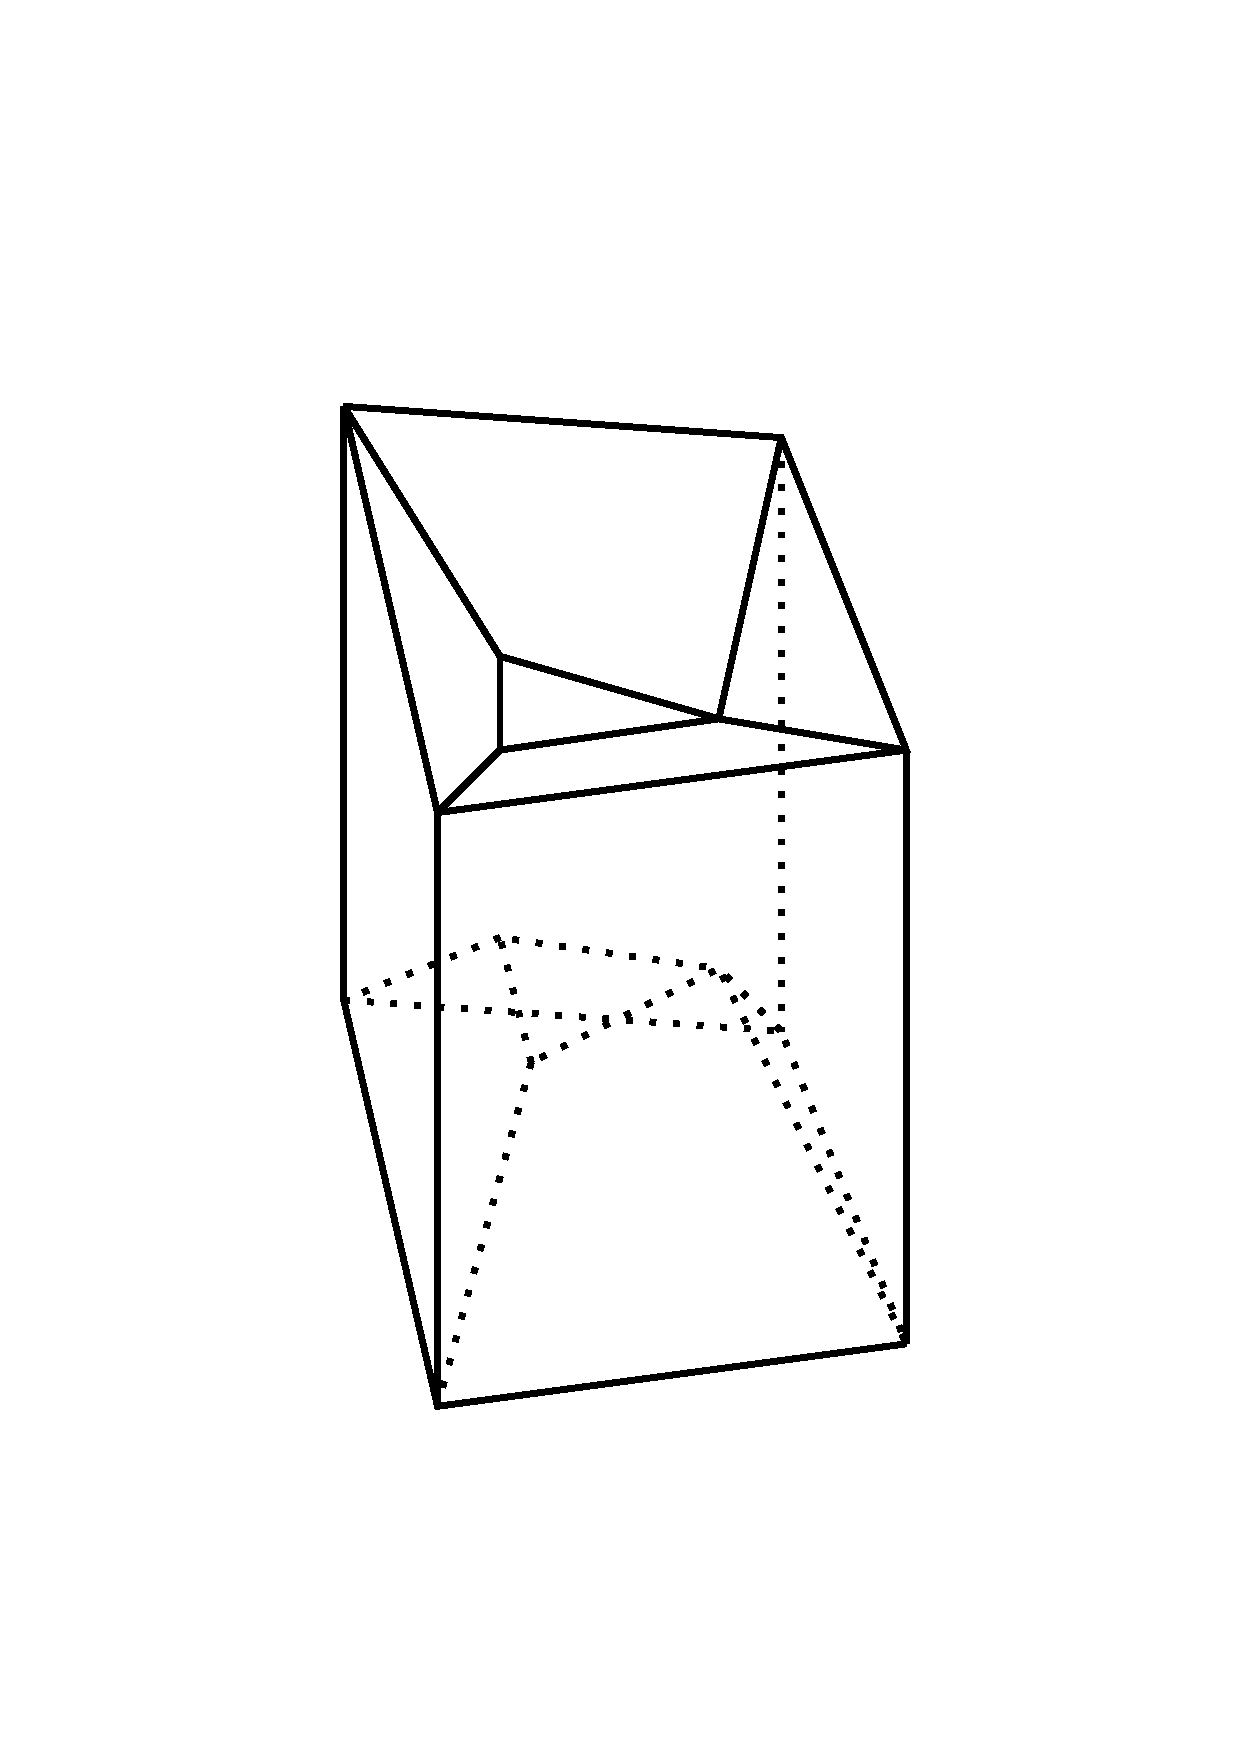
\includegraphics[width=\textwidth]{genus/genus-2}
        \caption{Triangles nearing.}
        \label{fig:decending-faces}
        \end{subfigure}
          \hspace{.5cm}
         \begin{subfigure}[b]{0.2\textwidth}
        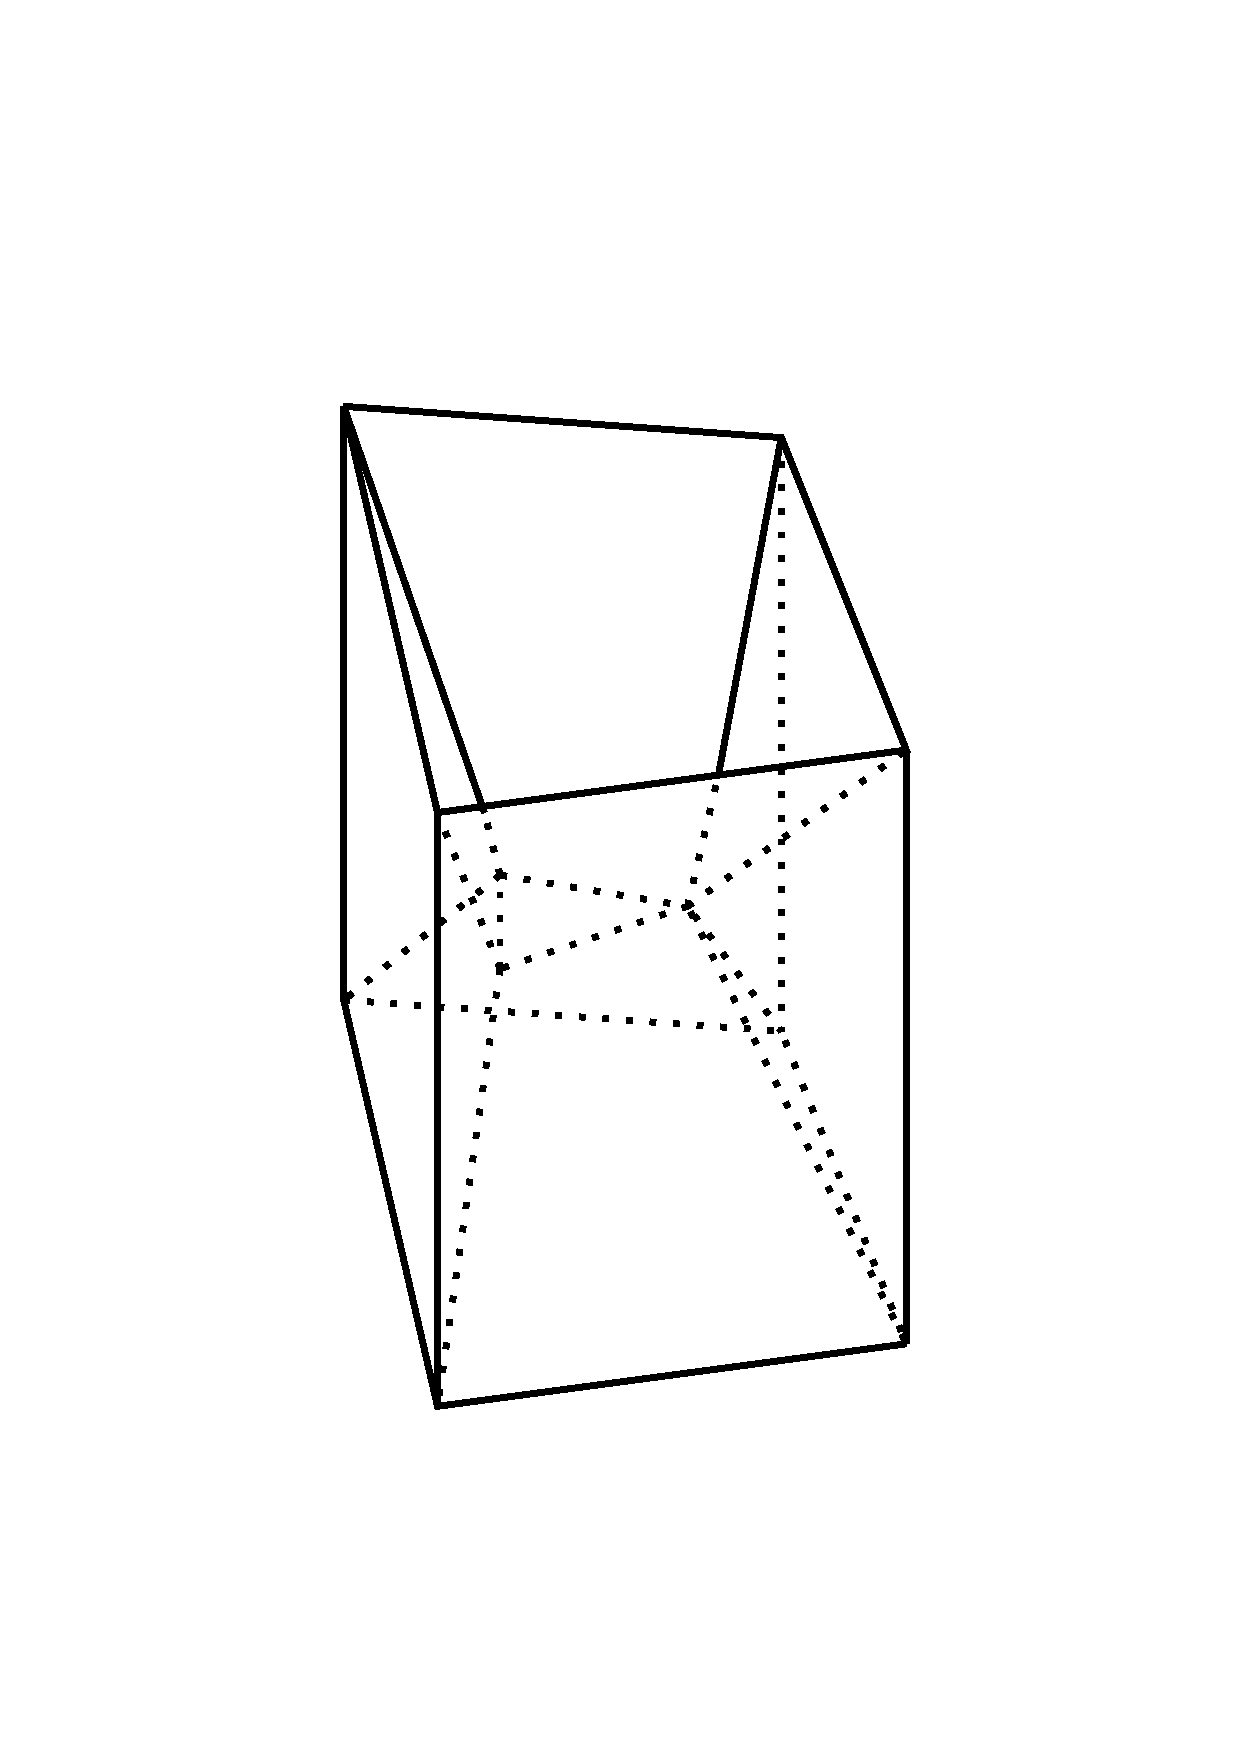
\includegraphics[width=\textwidth]{genus/genus-3}
        \caption{Triangles join.}
        \label{fig:faces-join}
        \end{subfigure}
		\caption{(\subref{fig:initial-sphere}) A surface homeomorphic to the sphere with genus zero.
		(\subref{fig:decending-faces}) The triangle on the top and the triangle on the bottom are getting
		closer. (\subref{fig:faces-join})  A surface homeomorphic to the torus. The triangle on the top
		and the triangle on the bottom have been removed. Three vertices and three edges have also been
		removed. The Euler characteristic decreased by two.
		\label{fig:genus}}
\end{figure}

\section{The Gauss-Bonnet Theorem}



The Gauss-Bonnet theorem for regular surfaces states

\begin{theorem}[The Continuous Gauss-Bonnet Theorem] \label{thm:g-b-c}

If $M$ is a regular surface with boundary $\partial M$ then
	$$\int_{M} K dA+ \int_{\partial M} k_g ds + \sum_i \beta_i= 2\pi \chi(M)$$
	where  $K$ is Gaussian curvature,
	 $k_g$ is the geodesic curvature,
	 each $\beta_i$  is an exterior angle at a vertex of the boundary and
	$\chi$ is the Euler characteristic.
\end{theorem}


The  Gauss-Bonnet theorem is  telling us, if we add up curvature
at each vertex the sum will be $2\pi$ times to Euler characteristic.
If we can compute the curvature at every vertex then we can use the theorem
to learn global topological information.
Conversely, if we know the Euler characteristic we can learn about the curvature
at individual points.

\subsection{Two Proofs}
We now include a proof of a combinatorial version of the theorem due to Banchoff
\cite{banchoff_critical_1970}
\todo{Choose a proof}
\section{A Discrete Version}
\label{sec:discrete}

In this section, we use the Gauss-Bonnet theorem to derive
a definition of discrete curvature. We discuss how discrete curvature
is used to improve meshes that are generated by scanning.
We then prove a discrete version of the Gauss-Bonnet theorem.

Consider a triangulated polygonal surface $S$ with boundary $\partial(S)$.
The boundary is a one dimensional piecewise linear curve in $\R^3.$
As with polygons in the plane, at each vertex $v\in \partial(S)$ 
we have an exterior angle.

The interior angle might consist of many triangles.
Let $F_v$  denote the set of faces incident to $v$ and let
$\alpha_f$ denote the angle in face $f$ at $v$.
The \EMPH{discrete geodesic curvature}
of $v$  is
$$k_{g}(v)= \pi-\sum_{f\in F_v}\epsilon_f.$$
See \figref{discrete-geodesic} for an illustration.
Notice that if $v$ lies on a straight line, then $\sum_{i}\epsilon_f=\pi$
and the curvature is zero as we would expect.


\begin{figure}[htb]
\centering
	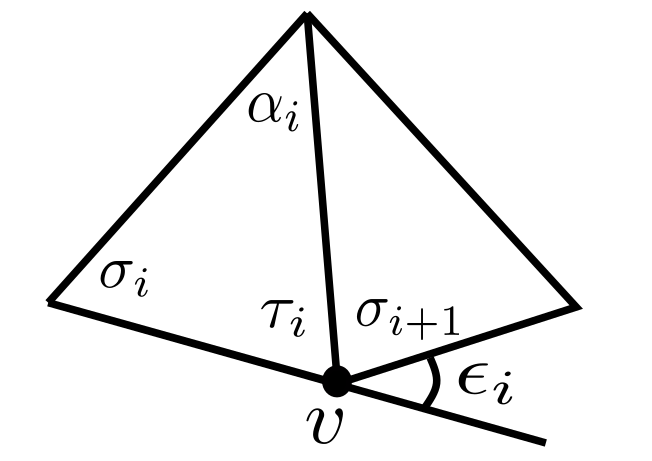
\includegraphics[width=.25\textwidth]{curvature/discrete-geodesic}
	\caption{The discrete geodesic curvature at a vertex $v$ on the boundary
	of a surface is given by the exterior angle $\epsilon$.}
	\label{fig:discrete-geodesic}
\end{figure}

How should be define discrete Gaussian curvature?
At every non-vertex point on a polygonal surface, the continuous Gaussian curvature
is zero and at every vertex it is undefined.
We can use the intuitive definition of discrete geodesic curvature and the Gauss-Bonnet
theorem to give a definition for discrete Gaussian curvature.

Consider removing the neighborhood around a vertex $v$ consisting
of the faces incident to $v$ and the edges and vertices of these faces call
this $N(v)$.
Using the variable names given in \figref{discrete-geodesic},
the total geodesic curvature

\begin{align}
\int_{\partial N(v)} kg ds &=\sum_i \pi -(\tau_i+\sigma_{i+1})\nonumber  \\
       &=\sum_i \pi -(\tau_i+\sigma_{I}) \nonumber  \\
       &=\sum_i \alpha_i. \nonumber 
\end{align}
Where the second equality comes from the boundary being a circle and reorganizing the sum.
Topologically, this neighborhood is a disk and $\chi(N(v))=1$
so the Gauss-Bonnet theorem tells us that 
the discrete Gaussian curvature at a vertex is
\begin{definition}[Discrete Gaussian curvature\footnote{Discrete Gaussian curvature
is also called the \emph{angle defect} at a vertex}]\label{def:discrete-curvature-vertex}

$$K(v)=\int_{N(v)}K da=2\pi-\sum_i \alpha_i.$$

\end{definition}

Recall, that when we considered the curvature at a vertex on a polygon in the plane
in the theorem of turning tangents, \thmref{simple-bonnet}, we have two parts depending on
weather we use the interior or the exterior angles at each vertex.
We can do a similar thing with the discrete Gaussian curvature at a vertex on a surface,
instead of considering the angles of the faces incident to a vertex $v$, we can consider
the complementary angle. The complementary angle is shown in \figref{switcheroo}. 
If we let $n$ be the number of faces
incident to $v$, the formula for the discrete curvature then becomes
\begin{equation}\label{eqn:discrete-curvature-complement-angle}
K(v)=2\pi - \sum_{i=1}^n (\pi - \xi_i)=(2-n)\pi +\sum_{i=1}^n \xi_i.
\end{equation}
By \eqnref{sphere-area}, this is the area of the polygon on the sphere with interior
angles $\xi_1, \xi_2,\ldots \xi_n.$
Geometrically, this angle be seen in \figref{switcheroo}.
If we project the normal vectors on each face onto a sphere and
connect these points with great arcs to create a polygon on the sphere with interior angles
$\xi_1, \xi_2,\ldots \xi_n.$
We have a geometric representation of discrete
Gaussian curvature as the area on the unit 
sphere bounded by a spherical polygon whose vertices are the unit normals of 
the faces around $v$. An example is shown in \figref{discrete-curvature}.

\begin{figure}[htb]
\centering
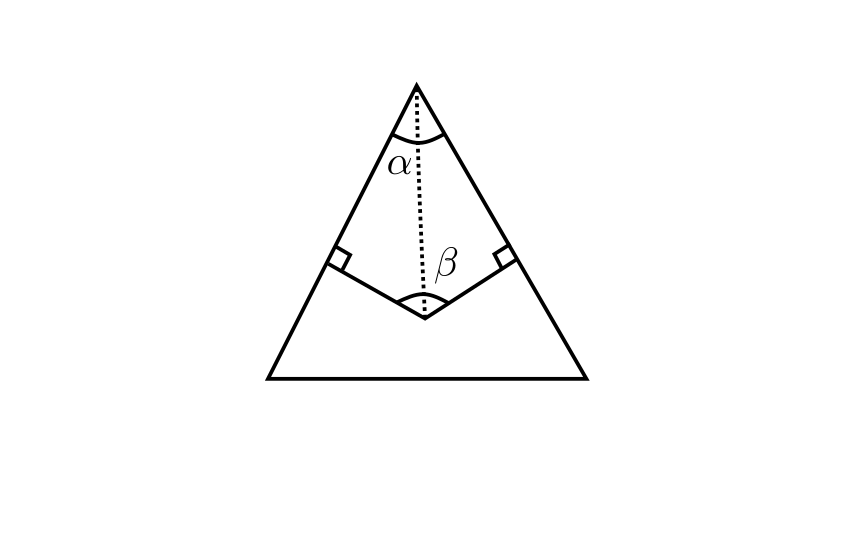
\includegraphics[width=.25\textwidth]{background/switch-angles}
\caption{The relationship between the angles incident to a vertex and
its complementary angle.}
\label{fig:switcheroo}
\end{figure}





\begin{figure}[htb]
\centering
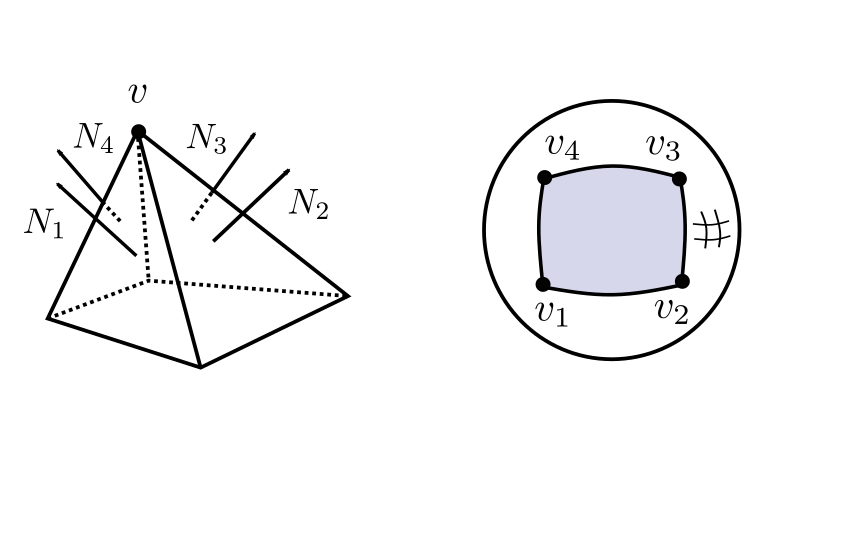
\includegraphics[width=.5\textwidth]{curvature/discrete-curvature}
\caption{Consider the vertex $v$ in the figure on the left. The curvature of $v$
is the area on the sphere shown on the right. We rotated the sphere
in order to see the entire polygon.}
\label{fig:discrete-curvature}
\end{figure}







Combining the above definitions  we have

\begin{theorem}[The Discrete Gauss-Bonnet Theorem] \label{thm:g-b-d}

If $S$ is a triangulated surface with  boundary $\partial S$ then
$$\sum_{v\in V_{int}} K(v) + \sum_{v\in V_{\partial S}} k_g(v) = 2\pi \chi(S)$$
where $K(v)$ is the discrete Gaussian curvature
of a vertex, $k_g(g)$ is the discrete geodesic curvature,  and
$\chi$ is the Euler characteristic.
\end{theorem}



\section{Reducing the Size of a Mesh}
\label{sec:removing}



Meshes that are obtained by scanning real objects contain noise.
Most meshes that are generated by scanning require a complete
remeshing \cite{remeshing-2003}.
As a first step in remeshing, the curvature at each
vertex needs to be estimated.

In \cite{mmsb-2003}, Meyer et al., define the gaussian curvature operator
to estimate the curvature at each vertex. Their operator is 
based on a simple application of the Gauss-Bonnet theorem.
The central idea is to cut a disk around each vertex that does not contain
any other vertices. Then, all Gaussian curvature in the removed
disk is occurs at the vertex of interest.

We associate an area around each vertex $v$. 
For each triangle incident to $v$, if the interior 
angle at $v$ is non-obtuse, mark the circumcenter of the triangle
and if the interior angle is obtuse, make the mid point of the edge
opposite of $v$. See \figref{mixed-area} for an illustration.
Denote the area of this polygon by $A_m.$


\begin{figure}[htb]
\centering
\includegraphics[width=.3\textwidth]{meshes/mixed-area}
\caption{The area $A_m$ associated with a vertex $v$.}
\label{fig:mixed-area}
\end{figure}


Then, since we are considering a closed two-disk $A$ we have $\chi(A)=1$.
Let $F_v$ denote the number of faces incident to $v$, 
then by the Gauss-Bonnet theorem we have

$$\int \int_{A_m}K dA +\sum_i^{F_v} \epsilon_i=2\pi$$
where the sum is over the faces incident to $v$.
The Gaussian curvature operator at a vertex $v$ is defined
to be
$$K(v)=\left( 2\pi -\sum_i^{F_v}\epsilon_i\right)/ A_m.$$

The experiments in \cite{mmsb-2003} found that the average
percent error did not exceed $1.3\%$ when using this operator.

Computing the curvature at each vertex in a mesh can allow one to reduce
the number of vertices in the mesh without sacrificing mesh quality.
This leads to more efficient algorithms and reduced storage space.
One example is given in \cite{alliez-2002},
Given a mesh, we compute the curvature at each vertex.
The number of points included in the re-mesh is determined
by the curvature. If the curvature is small, then few points
are sampled to be included in the re-mesh. If the curvature
is large, then many points are sampled. See \figref{planck-mesh}
for an illustration.

\begin{figure}[htb]
\centering
\includegraphics[width=.7\textwidth]{meshes/planck-mesh.jpeg}
\caption{A mesh of Max Plank. The original mesh is on the left. As we move
from left to right more importance is placed on vertices with large curvature.
Figure from \cite{alliez-2002}.}
\label{fig:planck-mesh}
\end{figure}

\subsection{A Combinatorial Proof}
\label{sec:proof}


We present a proof of the Gauss-Bonnet theorem similar to the proof given by Upadhyay \cite{upadhyay2015}.
First, we consider the case where our surface does not have a boundary.
We then extend this case to surfaces with boundary.
\begin{theorem}[Discrete surfaces without boundary]\label{thm:g-b-discete-bdy}
For a triangulated surface $S$ without boundary
$$\sum_{v\in V} K(v)=2\pi \chi(S)$$
where $K(v)$ is the discrete curvature.
\end{theorem}

\begin{proof}

For each vertex $v$ in $S$,
let $deg(v)$ denote the number of edges incident to $v$, let $\alpha_1,\alpha_2,\ldots,\alpha_{\deg{(v)}}$ denote the angles
containing $v$ and let $\xi_i=\pi-\alpha_i$ for each $i$.
By \eqnref{discrete-curvature-complement-angle}, 
the discrete Gaussian curvature at a $v$ is
 $$K(v)=(2-\deg{(v)})\pi +\sum_{i=1}^{\deg{(v)}} \xi_i.$$
Summing over all vertices in $S$ gives
$$\sum_{v\in V} K(v)=\sum_{v\in V}2\pi - \sum_{v\in V}\deg{(v)}\pi+\sum_{v\in V}\sum_{i=1}^{\deg{(v)}} \xi_i.$$
The first term on the right hand side is $2\pi |V|$. Each edge is incident with two vertices, so the second term is $2\pi |E|$. 
In the third term, we rewrite $\xi_i$ as $\pi-\alpha_i$.

$$ \sum_{v\in V}\sum_{i=1}^{\deg{(v)}} \beta_i= \sum_{v\in V}\sum_{i=1}^{\deg{(v)}} (\pi-\alpha_i).$$
We can reorganize this sum as follows, instead of summing the angles around each vertex we can sum the angles in each face.
Each angle in $S$ is still being counted exactly once. 
Since each face is a triangle, this gives
$$\sum_{v\in V}\sum_{i=1}^{\deg{(v)}} (\pi-\alpha_i)=\sum_{f\in F}\sum_{i=1}^3(\pi-\alpha_i).$$
Since each face is a triangle the sum of the three angles is $\pi$,
so $\sum_{i=1}^3(\pi-\alpha_i)=3\pi-\pi=2\pi.$
Thus, $$\sum_{v\in V} K(v)=2\pi |V|-2\pi |E|+2\pi |F|=2\pi \chi(S)$$ as desired.
\end{proof}

The above proof can be extended to the case where $S$ has a boundary
by gluing a copy of $S$ to itself along the boundary.

\begin{theorem}[Discrete surfaces without boundary]\label{thm:g-b-discete}
For a combinatorial surface $S$ with no boundary

$$\sum_{v\in S_{\text{int}}} K(v)+\sum_{v\in\partial S}k_g(v)=2\pi \chi(S)$$
where $k_g(v)$ is the exterior angle at $v$ 
$k_g(v)=\pi-\sum_i\alpha_i$ for $\alpha_i$ incident to $v$.
\end{theorem}

\begin{proof}
Take a copy of $S$ and attach it to itself along the boundary.
This creates the surface $2S$ without boundary. Notice,
when we copy $S$ we create two copies of the boundary, and when
we glue we remove one copy of the boundary.
Thus, $\chi(2S)=2\chi(S)-\chi(\partial S).$
Since, $\partial S$ is piecewise linear the number of vertices and
edges are equal and there are no faces, so $\chi(\partial S)=0$
and 

\begin{equation} \label{eqn:glue}
\chi(2S)=2\chi(S).
\end{equation}

For $v$ a vertex on the boundary, $k_g(v)$ is half
the discrete gaussian curvature of $v$ in $2S.$

Thus,

$$\sum_{v\in 2S}K(v)=2\left(\sum_{v\in S_{\text{int}}}K(v)+\sum_{v\in \partial S} k_g(v)\right) =2\pi  \chi(2S).$$
Applying \eqnref{glue},

$$\sum_{v\in S}K(v)+\sum_{v\in \partial S} k_g(v)=2\pi  \chi(S)$$
as desired.

\end{proof}
\section{Applications}\label{sec:applications}
\subsection{The Harry Ball Theorem}
\label{sec:harry-ball}

Functions on surfaces are called vector fields.
In this section, the Gauss-Bonnet theorem is used
to relate the zeros of a vector field to the topology of a surface.
We will prove that harry ball theorem which shows that 
given a harry ball, one
can not comb the ball without creating a cowlick.




\begin{definition}[Vector Field]\label{def:vector-field}
	A vector field $v$  on an open set $U\subset S$ of a regular surface $S$
	is a correspondence which assigns a vector $w(p)\in T_p(S)$ to each $p\in U$.
	Moreover, $v$ is differentiable at $p$ if, for some parametrization $r(u,v)$ at $p$,
	the functions $a(u,v)$ and $b(u,v)$ given by
		$$v(p)=a(u,v)r_u + b(u,v)r_v$$
	are both differentiable at $p$.
\end{definition}

A point $p\in S$ in vector field is a \EMPH{singular point} if $v(p)=0$
moreover, a singular point is \EMPH{isolated} if there is an open neighborhood
containing $p$ and no other singular points. These, and the following definition,
extend to higher dimensions.

Let $f:\Sp^n\to \Sp^n$ be a continuous map. Let $H_n(\cdot)$ dentote  
the $n$th  homology group, then $f$ induces a homomorphism
$f_*:H_n(\Sp^n)\to  H_n(\Sp^n)$ and  $H_n(\Sp^n)\cong \ZZ$.
 Every homomorphism from $\ZZ$ to itself is of the form $f_*:n\mapsto kn$ for some 
$k\in \ZZ$ the integer $k$ is the \EMPH{degree} of the map $f$.

Isolated singular points give a map from the circle to itself.
Let $\sigma$ be a circle surrounding a singular point $p$.
Since $v(p)$ is isolated we can choose the radius of $\sigma$ to be 
small enough so that $v|_\sigma\neq 0$. 
The \EMPH{index} of a isolated critical point $p$ of $v$ is the degree
of the map $f:\sigma\to \Sp^1$ where$f(p)=v(p)/||v(p)||$.





\begin{theorem}[Poincar\'{e}-Hopf Theorem]\label{thm:poincare-hopf}
	Let $S$ be a closed and bounded regular surface and let $v$ be a vector field
	on $S$ such that every zero of $v$ is isolated. If $S$ has a boundary, 
	then assume $v$ is outward normal on the boundary. Then
	$$\sum_iI(v_i)=\chi(S)$$
	where $v_i$ denotes the set of isolated zeros.
	
\end{theorem}

We now prove that given a ball with a hair attached to each point, you can not
comb the ball without creating a cowlick.

\begin{theorem}[The Harry Ball Theorem]\label{thm:harry-ball}
	Let $v$ be a vector field on the sphere $\Sp^2$.
	Then there is a $p\in \Sp^2$ such that $v(p)=\vec{0}$.
\end{theorem}

\begin{proof}
	For a contradiction, assume that $v(p)\neq 0$ for all  $p\in \Sp^2$,
	this would give a vector field on $\Sp^2$ with no singular points.
	However, the Euler characteristic of $\Sp^2$ is two and
	\thmref{poincare-hopf} implies that any vector field on $\Sp^2$ has at
	least two isolated singular points.
	
\end{proof} 
\cite{rotskoff2010}
\subsection{Robotics}
\label{sec:robotics}
In may 2023 I asked chatgbt to give me some applications of the Gauss-Bonnet theorem and returned
that there were applications to robotics. I asked for some references here is what is said
``Yes, here are some references for the applications of the discrete Gauss-Bonnet theorem to robotics: 1. “Geometric Mechanics Approach to Control of Superparamagnetic Beads in High-Throughput Robotic Platforms” by P. Szymczak, E. Garcia-Miralles, and S. Misra, IEEE/ASME Transactions on Mechatronics (2015). 2. “Geometric Path Planning for Robotics Using Discrete Gauss-Bonnet Theorem” by V. Sarma and B. Ravani, IEEE International Conference on Robotics and Automation (2011). 3. “Gaussian Curvature-Based Navigation Algorithm for Mobile Robots” by Z. Chen, X. Yan, and Y. Zhang, IEEE Transactions on Robotics (2012). 4. “A Curvature-Based Approach to Visual Servoing for Robotic Manipulators” by Y. Liu and G. Hu, IEEE Transactions on Robotics (2010). These references provide examples of how the discrete Gauss-Bonnet theorem and related geometric techniques can be used in robotics, including control of magnetic beads, geometric path planning, navigation algorithms, and visual servoing."

These references seem to be made up but some web searches lead me to the following
not made up application of the Gauss-Bonnet theorem in robotic 
route planning is given by K.-L. Wu et. al. in \cite{wu_path_2016}.
Suppose have a robot navigating a 3D\todo{2 or 3 manifold?} terrain with a single obstacle
and we wish to plan trips for our robot.
In this application, a terrain is a smooth manifold \todo{not defined} with tangent planes
at every point. An obstacle is modeled by a hazardous ball with a grade depending on the radius.
Assume that checking if a path intersects the obstacle can be done in constant time.


Overview of their procedure.
We are given two points $s$ and $t$ on a ?-manifold $M$.
First, compute a geodesic path from  $s$ to $t$ call this path $\gamma(x)$.
If the $\gamma$ does not intersect the obstacle we are done.
Otherwise, the $\gamma$ intersects the obstacle
we call the initial intersection point between our path
and the boundary of the obstacle $p$.
Construct the tanged plant $TpM$ at $p$.
Choose a vector $v\in TpM$ and a value $\alpha$ for the magnitude of $v$.
Next, define two points $\alpha_{\ell}$ and $\alpha_{u}$
to be in the directions of $v$ and $-v$ at a distance of $\alpha$
from $p$ in the tangent plane. Then project the points   $\alpha_{\ell}$ and $\alpha_{u}$
onto the surface? to obtain the points $q$ and $r$.
We next compute four new  geodesics $g_1(s)$ from $s$ to $q$,
$g_2(s)$ from $q$ to $t$, 
$f_1(s)$ from $s$ to $r$ and 
$f_2(s)$ from $r$ to $t$. Let $\gamma_g=g_2\circ g_1$ and $\gamma_f=f_2\circ f_1$.

We then use the Gauss-Bonnet theorem to decide which alternative path is best.
If the edges of a triangle are all geodesic then we have a \EMPH{geodesic triangle} $\tau\subset M$.
We have two geodesic triangles, $\gamma, g_1,g_2$ and $\gamma,f_1,f_2.$

Here we have cusps at the intersection points of the geodesics,
to account for this, our Gauss-Bonnet is 
\begin{equation}\label{eqn:b-g-angles}
\int \int_{\tau} K dA +\sum_{i=1}^3(\pi-\theta_i)+\sum_{i=1}^3 \int k_gds =2\pi
\end{equation}
where $\theta_i$ are the interior angles of $\tau$.
Since we are on geodesics $\int kgds =0$ and we can rearrange
\eqnref{b-g-angles} to obtain

\begin{equation} \label{eqn:interior-angles}
\theta_1+\theta_2+\theta_3 = \pi +\int \int_{\tau} K dA.
\end{equation}

We can estimate the curvature based on the sum of the angles of
$\sum_{i=1}3\theta$.
They show that f $K=0$ on $\tau$ then $\gamma_f$ and $\gamma_g$
are identical and there exists an $\alpha^*$ that makes them shortest.
If $\sum_{i=1}3\theta_i>\pi$ then is $\int_?K>0$ on all of $\tau$ then and if $\sum_{i=1}3\theta_i<\pi$
then $K<0$ on (average) all of $\tau$.
The authors state that we should avoid negative curvature because it
is ``energy-consuming ascending and descending motions required"
and would require the robot have ``better mobility and maneuverability".
\todo{I don't see why}.



\section{How Many Deltahedron Exist?}
\label{sec:deltahedron}

In this section, we share a proof due to
Fushsida-Hardy \cite{deltahedron} that there are
only eight deltahedron.

A \EMPH{deltahedron} is a polyhedron whose
faces are all equilateral triangles.




\subsection{Pseudosphere}
\label{sec:pseudosphere}

The sphere is a surface with constant positive curvature.
Are there surfaces with constant negative curvature?
The answer is yes, one such surface is the pseudosphere
which we introduce here. We will then use the Gauss-Bonnet
theorem to determine the Euler characteristic of the pseudosphere as
shown in \cite{pseudo-app}.


The tractrix is the curve whose tangent meet the $x$-axis a unit distance
from the point of tangency \cite{thurston}. See \figref{tractrix} for an illustration.
Intuitively, imagine a bike with unit distance between where the tires meet the ground.
Place the back wheel on the positive $y$-axis and front wheel on the origin pointed
toward the positive $x$-axis. We then push the bike forward while keeping the front
wheel on the $x$-axis. Then do the same in the negative $x$ direction.
The tractrix is the curve traces by the back tire. 


\begin{figure}[htb]
    \captionsetup[subfigure]{justification=centering}
    \centering
    \begin{subfigure}[b]{0.4\textwidth}
        \includegraphics[width=\textwidth]{pseudosphere/tractrix}
       \subcaption{}\label{fig:tractrix}
    \end{subfigure}
        \hspace{1cm}
        \begin{subfigure}[b]{0.4\textwidth}
        \includegraphics[width=\textwidth]{pseudosphere/pseudosphere}
        \subcaption{}\label{fig:pseudosphere}
        \end{subfigure}
    \caption{(\subref{fig:tractrix}) The length of the tangent vector from a point to the $x$-axis is one.
        (\subref{fig:pseudosphere}) The truncated pseudosphere.
    }
    \label{fig:tractrix-pseudosphere}
\end{figure}



The pseudosphere is the surface formed by rotating the tractrix around the $x$-axis.
An example is shown in \figref{pseudosphere}.
One can show that the curvature of a surface of revolution formed by rotating a curve
$(x(t),y(t)),$ where $t$ is the arc length, about the $x$-axis is given by

$$K=-\frac{1}{y}\frac{d^2t}{dt^2}$$
and conclude that the curvature is negative one.
Using the well know formula for the surface area of a surface of revolution
we see that the area of the pseudosphere is $4\pi$.

Suppose we wish to compute the Euler characteristic of half of the pseudosphere,
the Gaussian curvature is $-1$ and the area is $2\pi$, we need to compute
the geodesic curvature of the boundary. 

The boundary occurs where $x=0$, we should also consider what happens as $x$ approaches
infinity.  When $x=0$ the boundary is a unit circle 
$$c(t)=(\cos(t),\sin(t),0),$$ using the \eqnref{geodesic}, we have
$$k_g=\langle c''(t),(N\times c'(t))=1.$$
Plugging into the Gauss-Bonnet theorem we see that
the Euler characteristic of the top half of the pseudosphere is zero!




\section{Triangulating Noncovex Polyhedra}
\label{sec:triangulating}

Discrete three-manifolds are called \EMPH{polyhedra}. 
A polyhedron is \EMPH{simple} if it is homeomorphic to the sphere 
and the faces are all polygons.
Let $P$ be a a simple polyhedron.
A triangulation of a three-manifold is a decomposition
of $P$ into tetrahedra.
Often, we wish to represent the three-manifold
with as few tetrahedra as possible \cite{simplify-mesh-1999}.
Let $n$ be the number of vertices in a simple polyhedron,
in the worst case, decomposing the $P$
 into tetrahedra requires $\Omega(n^2)$ tetrahedra
\cite{chazelle-lower-1984}.

 An edge $e$ in $P$ is
\EMPH{reflex} if the interior angle formed by its two incident faces
is greater than $\pi$.
A vertex is reflex is it is incident to a reflex edge.
Let $r$ denote the number of reflex edges.
See \figref{reflex} for an example.

\begin{figure}[htb]
\centering
\includegraphics[width=.3\textwidth]{meshes/reflex}
\caption{A polyhedron with one reflex edge (blue), the two vertices incident to the blue
edge are reflex vertices.}
\label{fig:reflex}
\end{figure}
Chazell and Palios give an
algorithm to triangulate a nonconvex simple polyhedra \cite{triangulating-polytope-1990}.
 Their algorithm creates a refinement with $O(n+r^2)$ tetrahedra
in $O(n\log r +r^2\log r)$ time and $O(n+r^2)$ space.
The algorithm first removes $n-4r$ non-reflex or flat vertices
to create a representation of the polyhedra with $O(r)$ vertices.
Then, vertical planes decompose the reduced polyhedra in to
$O(r^2)$ convex cells.

Chazelle and Shouraboura use the Gauss-Bonnet theorem to show any polyhedron
 of genus $g$ must have at least $g-1$ reflex edges~\cite{tetra-bounds-c-s-1994}.
 This implies that any polyhedron
can be decomposed with $O(n+r^2)$ tetrahedra, regardless  of 
the genus!  We present their application.

In this application, to simplify computation we scale the curvature of a vertex
by $\frac{1}{2\pi}$, so be $k_v=\frac{1}{2\pi}\left(2\pi-\sum_i \alpha_i\right)$,
First, we show 

\begin{lemma}\label{lem:reflex-edge}
The number of reflex edges  incident to a vertex $v$  is at least $-k_v.$
\end{lemma}

\begin{proof}

For each vertex, center a sphere at the vertex,
see \figref{sphere-on-vert}.
The intersection of the polyhedron and the sphere
gives a `polygon' on the sphere with boundary $L$ consisting of great
circles. 
Scale the sphere to have unit radius. Then, the length of each arc
in $L$ is equal the the angle incident to $v$, so the total length of $L$ is
the sum of the angles incident to $v$, see \figref{sphere}.

Let $R$ be the number of reflex edges incident to $v$.
If $R$ is zero, then $P$ is convex and has non-negative curvature
so $L\leq 2\pi$. If $R>0,$
reflex edges incident to $v$ correspond to reflex angles in $P$.
If we have a reflex angle in $P$, bisect it and reduce the 
number of reflex angles and obtain a decomposition
of the sphere into at most $R+1$ convex regions,
thus $L\leq 2\pi(R+1)$.

Thus, we have $L=\sum \alpha_f$ and the curvature 
$k_v=2\pi-\sum \alpha_f$ giving
$L=2\pi(1-k_v)$. Combining this with $L\leq 2\pi(R+1)$
gives $-k_v\leq r.$


\end{proof}

\begin{figure}[htb]
        \centering
        \begin{subfigure}[b]{0.35\textwidth}
        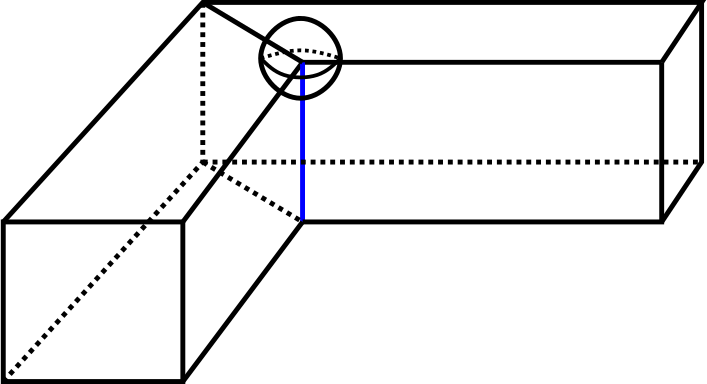
\includegraphics[width=\textwidth]{meshes/reflex-vert-sphere}
        \caption{}
          \label{fig:sphere-on-vert}
        \end{subfigure}
          \hspace{.0cm}
         \begin{subfigure}[b]{0.45\textwidth}
        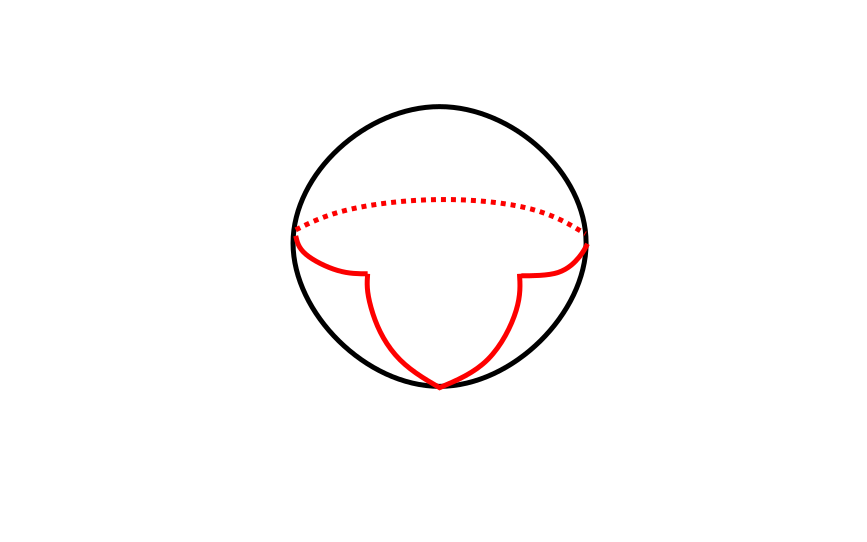
\includegraphics[width=\textwidth]{meshes/sphere-intersection}
        \caption{}
        \label{fig:sphere}
        \end{subfigure}\\
		\caption{(a) A sphere centered at a reflex vertex. (b) The `polygon'
		of great circles where the polyhedron intersects the sphere. 
		\label{fig:sphere}}
\end{figure}


Next, we show
\begin{theorem}[Reflex Angles]\label{thm:reflex}

Any polyhedron of genus $g$ must have 
at least $g-1$ reflex dihedral angles. 

\end{theorem}
\begin{proof}
Let $r$ be the total number of reflex edges in a polyhedra.
By the classification of oriented surfaces, the Euler characteristic 
 is determined by the genus, $\chi=2-2g$.
By \lemref{reflex-edge}, $\sum_v -k_v\leq 2 r$ since each
reflex edge is incident to two vertices.
By the Gauss-Bonnet theorem $\sum_vk_v= 2-2g,$
so $-2r\leq 2-2g$ and $g\leq r+1$ as desired.

\end{proof}

Given a polyhedron of genus $g$, we can temporally 
duplicate the vertices around each essential cycle and insert disks,
 creating a polyhedron of genus zero, we theb apply the algorithm to
decompose genus zero polyhedra given in \cite{triangulating-polytope-1990}.
Then remove the added disks.
Since we added $g$ disks the algorithm decomposes
the polyhedron into $O(n+ (r+g)^2)$ tetrahedra.
By \thmref{reflex}, $g\leq r+1$ showing that the upper bound
on the number of tetrahedra in a triangulation
of a polyhedra is $O(n+r^2)$ regardless of the genus.


\subsection{Digital Topology}
\label{sec:digital-topology}

Digital images consist of arrays of cubes.
Each cube is either black or white.
Given a digital image, one would like 
a computer to to classify the image.
Operations toward image classification include
object counting, border following and computing 
the homology of objects \cite{kong_digital_1989}.
Decomposing a cubical complex into a simplicial complex
results in 24 times as many highest dimensional cells \cite{Kaczynski2003}.


The elements of two-dimensional digital images
are \EMPH{pixels} and the elements of a three-dimensional
digital image are called \EMPH{voxels}.
Each pixel can be associated with a point in a lattice.
Two points in the lattice are four-adjacent if
they are  distinct and differ in at most one of their
coordinates, they are eight-adjacent
if they distinct and each coordinate entry differs by at most one.
In three dimensions, two points
are 26-adjacent if they are distinct and each coordinate 
entry differs by at most one.

If a set of points $S$ lattice points cannot be
partitioned into two subsets that are not
$n$-adjacent is \EMPH{$n$-connected}.

Consider four vertices adjacent to a single vertex $v$.
If four-adjacency is used the four black points are disconnected,
but separate $v$ from the exterior, if eight-adjacency is used
the back points form a Jordan curve that does not separate
an interior. To resolve this matter, we use eight-adjacency
for the white vertices and four-adjacency for the black.
We make a similar choice in three-dimensions.

\begin{figure}[htb]
        \centering
        \begin{subfigure}[b]{0.35\textwidth}
        \includegraphics[width=\textwidth]{digital/paradox}
        \caption{}
          \label{fig:paradox}
        \end{subfigure}
          \hspace{.0cm}
         \begin{subfigure}[b]{0.40\textwidth}
        \includegraphics[width=\textwidth]{digital/6-26}
        \caption{}
        \label{fig:6-26}
        \end{subfigure}\\
		\caption{(a) Are the black points a closed curve? (b) In three-dimensions,
		the six neighbors of the vertex $p$ are in pink and the 26 neighbors are in
		blue. 
		\label{fig:adjacency}}
\end{figure}

A \EMPH{digital picture} is a quadruple $(V,m,n,B)$ where
$V=\R^2$ and $(m,n)=(4,8)$ or $V=\R^3$ and $(m,n)=(6,26)$
and $B$ is a subset of $V$. Elements of $B$ are black vertices
and elements not in $V$ are white.

In \cite{chen_digital_2010}, Chen and Rong an
algorithm to compute the homology groups of a three dimensional
digital object in $\R^3$. Their algorithm uses the Gauss-Bonnet theorem
and is linear in the size of the input.


We consider cubical spaces in $\R^3$ with $(6,26)$-connectivity,
where two points are adjacent  if their Euclidean distance is 1.
If $M$ is a closed, orientable digital surface, there are
six types of digital surface points, these are shown in \figref{surface-points}.

\begin{figure}[htb]
        \centering
        \includegraphics[width=.45\textwidth]{digital/surface-points}
		\caption{
		\label{fig:surface-points}}
\end{figure}

Let $M_i$ denote the set of digital points with $i$ neighbors and $K_i$
the curvature.
Then, by \eqnref{defect}, we have
\begin{enumerate}[(a)]
\item $K_3=\pi/2,$
\item $K_4=0,$
\item $K_5=-\pi/2,$
\item $K_6=-\pi.$
\end{enumerate}

For a closed two-manifold the is the boundary of a three-dimensional
digital image, the Gauss-Bonnet theorem implies
$$\sum_{i=3}^6K_i |M_i|=2(2-2g).$$
A linear time algorithm to compute the genus is the following.
Iterate through all points in $M$ and count the neighbors at each point
and keep track of $M_i$. Then use the above equation to  calculate the genus
using 
$$g=1+(|M_5|+2|M_6|-|M_3|)/8.$$
\section{Homotopy Testing}
\label{sec:homotopy}

Homotopy classes of curves are important  because...
In this section, we share applications
where the Gauss-Bonnet theorem is used to determine
if curve on a surface is contractible.
An explanation of this algorithm is given in a video lecture 
by Jeff Erickson \cite{erickson-lecture}.

\begin{figure}[htb]
\centering
\includegraphics[width=.3\textwidth]{homotopy/contractable}
\caption{The blue curve is not contractable, the red curve is contractable.}
\label{fig:contractable}
\end{figure}

In this application, we will use a modified version
of the Gauss-Bonnet theorem. Given a combinatorial surface
$S$ define the curvature of a face to be $k(f)=1-\sum \beta_f$,
$k(v)=1-\frac{1}{2}\deg(v)+\sum_{v\in V} \alpha_v$.
Summing over all faces and vertices in $S$ gives,
\begin{theorem}[Modified Gauss-Bonnet]\label{thm:modify-g-b}
For a combinatorial surface $S$,
$\sum_{f\in F} k(f)+\sum_{v\in V}k(v)=\chi(S).$
\end{theorem}

\begin{proof}

$$\sum_{f\in F} k(f)+\sum_{v\in V}k(v)=|F|-\sum_{v\in V}\alpha_v + |V|-|E|+\sum_{v\in V}\alpha_v=\chi(S).$$
\end{proof}


Here, a we have a combinatorial surface that we call a map denoted $S$
with genus $g\geq 2.$ The case $g=0$ is the sphere where every curve
is contractible and when $g=1$ contractibility can be determined by a counting
argument\todo{explain}.
A curve is a closed walk, given as alternating sequence of vertices
and edges in $S$.
A \EMPH{homotopy} between two closed curves $\gamma_1$ and $\gamma_2$ that 
share a point $p_0$ is a continuous map $H\colon [0,1]\times \Sp^1 \to \mathbb{R}^2$ 
such that $H(0,\cdot)=\gamma_1$, $H(1,\cdot)=\gamma_2$, and $H(s,0)=p_0=H(s,1)$.

On a combinatorial surface, homotopies can be decomposed
into discrete moves called edge spikes, edge unspikes  and face flips.
The question we consider is: Given a closed walk $W$ in a map $\Sigma$ is there a finite
sequence of moves that reduces the curve to a trivial walk?


First, we transform $S$ into a simpler object called a system of loops.  
Let $T$ be a spanning tree of $S$, let $C$ be the edges in a co-tree
(a spanning tree of the dual), and let $L$ denote the left over edges,
Each edge in $S$ is in one of $(T,L,C)$.
Contract edges in $T$, delete edges in $C$ a system of loops $\Delta$.
When we contract and delete edges in $S$ we might affect edges in our walk $W$.
If we contract an edge in $W$, delete the edge from $W$.
If we delete and edge $e\in W$, face flip to avoid the deleted edge.
Get a new walk $W' \in \Delta$ homotopic to $W\in \Sigma$
now only haveing one vertex. Then, $W'$ has one vertex
with degree $4g$, one face with $4g$ edges, and $2g$ loops.
The length of the walk increases by at most $2g$.


The universal covering space of $S$ denoted $U$ is a plane
and when $g\geq 2$ $U$ has a natural hyperbolic geometry,
tiled by $4g$-gons.


Big idea: a curve is contractible closed walk in $S$
if and only if the walk is closed $U$.
Thus, our problem is equivalent to the following: Given a walk
in the universal cover of a system of loops, is it closed?

Here the walk is given as a starting vertex then we have a list of which
edges to take at each intermediate vertex. 
All vertices look the same, so we must determine if we have ended where
we began. 

Look for spurs or taking and instances where we talk the long way around a face, 
shorten the walk.
Any nontrivial contractible cycle contains either a spur or a bracket \cite{gertsen-short-1990}.
\begin{lemma}[Dehn's Lemma]\label{lem:dehn}
If $g\geq 2,$ then any nontirival closed walk has either a spur
or $4g-2$ consecutive edges on the boundary of a face.
\end{lemma}
\begin{proof}
Sketch: 
Any nontrival closed walk bounds a disk $D$ with $\chi(D)=1$, by the Gauss-Bonnet theorem
$$\sum_v k(v)+\sum_f k(f) =1.$$

Each face has $4g$ edges, each internal vertex has degree $4g$
and each  boundary vertex  has degree less than $4g$.
The angle of each angle on a face  is $\frac{1}{4}$,
thus, $k(f)=1-g<0,$ for internal vertices  $k(v)=1-g<0$ and for all
vertices on the boundary, $k(v)=\frac{3}{4}-\frac{\deg(v)}{4}$.
Boundary vertices fall into three  categories: convex, where $k(v)=\frac{1}{4}$
flats,  where $k(v)=0$  and concave where $k(v)<0$.

By G-B, $$|F|(1-g)+|v_{convex}|\frac{1}{4}\geq 1$$
and 
$$|v_{convex}|\geq (4g-4)|F|+4.$$

We divide by $|F|$ to determine the average number
of convex vertices per face to be greater than $4g-4$.
Thus, there exists some face that has $4g-3$ consecutive edges in the walk.
\end{proof}

This gives an algorithm for determining if a walk is closed in the universal
covering space.
Look for spurs and long boundary subpaths, the walk is closed if and  only if
we can  shrink the curve.
Label edges, walk is a sequence of labels
look at intervals of $4g-2$ in a walk, $8g$ paths
that represent long boundary paths, $4g$ spurs.
Slide window and look for spurs or long boundary paths.
If you find one remove it.

Brute force $O(g^3\ell)$ overall.
Can speed it up with Erickson DFA  idea
$O(g^2+g\ell)$.
Overall runtime $O(n+g^2+g\ell)$ time.

In trouble if $g$is big. Erickson uses system of quads,
radial map, $O(n)$ runtime  \cite{erickson-whittlesey-2013}.






\input{body/fta}


{
\small
\bibliographystyle{abbrv}
%\bibliographystyle{plainurl}
\bibliography{references}
}
\end{document}

